\documentclass[12pt,a4paper,twoside]{scrartcl}		% KOMA-Klassen benutzen!

%\usepackage[ngerman]{babel}			% deutsche Namen/Umlaute
\usepackage[utf8]{inputenc}			% Zeichensatzkodierung
\usepackage{url}
\usepackage{graphicx}
\usepackage{amsmath}
\usepackage{multicol}
\usepackage{glossaries}
\usepackage{expdlist}
\usepackage{subfig}
\usepackage{listings}
% see http://tex.stackexchange.com/questions/35145/maintaining-layout-of-tikz-diagrams-with-tex4ht-converting-as-single-pictures
\ifx\HCode\UnDef\else\def\pgfsysdriver{pgfsys-tex4ht.def}\fi
\usepackage{tikz}
  \usetikzlibrary{positioning,arrows,fit}
  \usetikzlibrary{decorations.pathmorphing,backgrounds,fit,decorations.pathreplacing}

\usepackage{setspace} % Anderthalbfacher Zeilenabstand ist Standard in den meisten Seminararbeiten. Das Paket setspace ermöglicht ein einfaches Umstellen von normalem, anderthalbfachen oder sogar doppeltem Zeilenabstand. 
\usepackage[paper=a4paper,inner=40mm,outer=30mm,top=25mm,bottom=25mm]{geometry} %Das geometry Paket dient zur Einrichtung der Seiten. Hier werden die jeweiligen Seitenränder angegeben. Diese wWerte sollten durch die jeweiligen Vorgaben des Seminarleiters oder Instituts ersetzt werden.
\setlength{\parindent}{1.0em} %Neue Abschnitte werden mit hängendem Einzug gesetzt, parindent definiert. um wie viel der Absat eingerückt wird. Die Einheit em ist abhängig vom verwendeten Zeichensatz und daher absoluten Werten in mm oder cm vorzuziehen. 
\setcounter{secnumdepth}{3} %Bis zu welcher Gliederungsebene nummeriert werden soll gibt dieser Befehl vor. In Falle 3 werden \section, \subsection und \subsubsection nummereiert.
\setcounter{tocdepth}{2} %Bis zu welcher Ebene Einträge ins Inhaltsverzeichnis aufgenommen werden. In diesem Beispiel ebenfalls bis Ebene drei (\subsubsection). Ein durch \paragraph ausgewiesener Abschnitt wird demnach nicht im Inhaltsverzeichnis auftauchen. 

\usepackage[colorlinks=false, pdfborder={0 0 0}, plainpages=false]{hyperref}

% http://tex.stackexchange.com/questions/9497/start-new-page-with-each-section
\usepackage{titlesec}
\newcommand{\sectionbreak}{\clearpage}

\usepackage{tocbibind}

\newcommand{\citeurl}[2]{\url{#1} (#2)}

\begin{document}

\lstnewenvironment{javalisting}[1][]
  {\lstset{language=Java,float=tb,#1}}% \begin{javalisting}[...]
  {} % \end{javalisting}

\lstnewenvironment{anylisting}[1][]
  {\lstset{float=tb,#1}}% \begin{anylisting}[...]
  {} % \end{anylisting}

\lstset{ %
  language=Java,
  float=tb,
  frame=single,
  captionpos=b
}

%\titlehead{}
%\subject{subject}

% Entwicklung einer REST-konformen Schnittstelle für die Opensource-Groupware
% Kolab mit Unterstützung verschiedener Medientypen

\title{A REST API for the Groupware Kolab with support for different Media Types}

\subtitle{bachelor thesis}

\author{Thomas Koch}
\publishers{Fernuniversität Hagen\\Faculty of mathematics and computer science}
\date{\today}

\maketitle{}
\thispagestyle{empty}
\pagenumbering{Roman}
\vspace{3cm}
\begin{center}
  matriculation number 7250371
\end{center}
\vspace{3cm}
\begin{center}
Professor Dr.-Ing. Bernd J. Krämer\\
Dipl.-Inf. Silvia Schreier
\end{center}

\section*{Aufgabenstellung}

\textit{Entwicklung einer REST-konformen Schnittstelle für die 
Opensource-Groupware Kolab mit Unterstützung verschiedener Medientypen}

Für die Opensource-Groupware Kolab\footnote{\url{http://kolab.org}} gibt es
bisher ein PHP-basiertes Web-Frontend. Als Alternative dazu soll eine
REST-konforme
Schnittstelle\footnote{\url{http://www.ics.uci.edu/~fielding/pubs/dissertation/top.htm}}
für die Kontaktfunktionalität entwickelt werden. Um die Anbindung an
verschiedene Clienten zu unterstützen sollen die folgenden Medientypen
unterstützt werden:

\begin{itemize}
\item
  vCard\footnote{\url{http://datatracker.ietf.org/doc/draft-ietf-vcarddav-vcardrev/?include_text=1}}:
  Für die Darstellung von Kontaktdaten eignet sich vCard, auch hier muss
  untersucht werden inwiefern die Daten aus Kolab abgebildet werden können.
\item Contact Schema von
  portablecontacts.net\footnote{\url{http://portablecontacts.net/draft-spec.html}}:
  Dieses JSON-Format, das auf vCard basiert, findet inzwischen auch in Open
  Social\footnote{\url{http://docs.opensocial.org/display/OS/Home}} Verwendung.
% Link für XHTML?
\item XHTML: XHTML eignet sich primär für menschliche Clients und kann beliebige
  Daten enthalten. Hierbei soll auch untersucht werden, inwiefern die Daten mit
  Hilfe von Microdata angereichert werden können, so dass dieses Format auch für
  maschinelle Clienten nutzbar wird.
\end{itemize}

Bei der Implementierung soll untersucht werden, welche Komponenten des Entwurfs
für die Unterstützung verschiedener Medientypen gemeinsam genutzt
bzw. wiederverwendet werden können. Außerdem soll die Hypermediaunterstützung
der verschiedenen Formate untersucht werden: Wie viel muss ein Client vorher
wissen und wie viel kann er durch Hyperlinks entdecken?

optionale Ergänzungen:

\begin{itemize}
\item CardDAV als alternatives Protokoll mit Untersuchung der
  Wiederverwendbarkeit der Komponenten
\item Mitbetrachtung der Kalenderfunktionalität bei der Hypermediaunterstützung
\item zumindest lesender Zugriff auf die Kalenderfunktionalität über die
  REST-Schnittstelle
\end{itemize}

\tableofcontents{}

\begin{abstract}
  % two or three short paragraphs (100-150 words total) background, project aims
  % and main achievements. From the abstract a reader should be able to
  % ascertain if the project is of interest to her and presents results that she
  % would like to know the details of
  % Hintergrund, Motivation, Ergebnisse
\end{abstract}
\newpage{}
\pagenumbering{arabic}



\section{Introduction}
\label{sec:introduction}

% Die Einleitung führt zum Thema hin. In der Einleitung muss deutlich werden, welche Frage Sie sich
% und dem Leser beantworten wollen und mit welcher methodischen Vorgehensweise dies
% geschehen soll. Nach der Lektüre der Einleitung sollte der Leser wissen, was ihn erwartet. Er kennt
% die Frage, er weiß in groben Zügen, wie Sie die Frage beantworten wollen, und er ist an der
% Antwort interessiert. Zum Abschluss der Einleitung sollten Sie eine kurze Übersicht über die
% nachfolgenden Kapitel geben.

% Einleitung (ca 2 Seiten)
% - Ziel der Arbeit
% - Beschreibung der Aufgabenstellung
% - Einbettung des Themas in ein größeres Umfeld
% - Anreize zum Lesen geben – keine Ergebnisse präsentieren
% - Kurze Beschreibung der einzelnen Kapitel (max. 1-3 Sätze/Kapitel)

Although computers became ubiquitous for some time now, they still don't help
their users with their most basic information management needs: Make contacts,
calendars, notices and to do items available across different devices and share
them with family and peers.

Most existing solutions are either based on non-free software (Microsoft Outlook),
or require the user to trust his personal data to the commercial
interests of a multinational corporation.
%\footnote{Experiences with Android and Data in the cloud \citeurl{http://keithp.com/blogs/calypso}{?}}

\section{Background and Related Work}
\label{sec:backgr-relat-work}

\subsection{REST architectural style}

The API to be designed in this work must obey the constraints of a REST
architecture, especially its four interface
constraints\cite[sec. 5.1.5]{Fielding2000}:

\begin{itemize}
\item Every resource is referenceable by a unique URI.
\item Resources are manipulated by the submission of resource representations.
\item All exchanged messages are self-descriptive which is achieved by using a
  set of Mediatypes understood by server and client.
\item The client only knows the entrance URI of an API beforehand. All other
  permitted URIs are discovered in responses of the server.
\end{itemize}

These constraints are further discussed in \autoref{sec:fieldings-critique} when
discussing how the OpenSocial API violates them.

The requirement to obey the constraints of REST should cause the system to have
some characteristics that may be especially advantageous for the use case of a
Groupware API. Those characteristics are, according to \cite{Fielding2000}
(cited sections in parentheses):

\begin{itemize}
\item Cacheability (sec. 5.1.4) can keep the data available also in offline
  mode, which improves performance and scalability.
\item Simplicity (sec. 2.3.3) helps to integrate the Groupware with other
  applications, e.g. publishing birthdays of employees in an intranet portal.
\item Modifiability (sec. 2.3.4) allows to adapt the Groupware to changes in the
  organization.
\item Reliability (sec. 2.3.7) can be of great importance, if the ability to
  work depends on the correct working of the Groupware system.
\item Anarchic scalability (sec. 4.1.4.1) allows a Groupware to function with
  other components that are not under the control of the Groupware
  administrator.
\end{itemize}

% Other outcomes described by Fielding that may not be of importance for the
% present work are: scalability in terms of users, network performance and
% efficiency.

\subsection{Kolab}
\label{sec:kolab}

``Kolab Groupware'' is the name for a system comprising several independent free
software products, a relatively small amount of Kolab specific ``glue code'' and
a special way to configure the involved components. On the server side, Kolab's
main components are the directory server OpenLDAP, the Mail Transfer Agent
Postfix and the IMAP server Cyrus. Kolab works with specialized client software
(see \autoref{sec:imap-as-collection}) which is officially available as free
extensions to KDE Kontact, Gnome Evolution and the PHP web clients Horde and
Roundcube.

The development of Kolab started 2002, when the Federal Office for Information
Security (Bundesamt für Sicherheit in der Informationstechnik) commissioned the
development of a free alternative to the Microsoft Exchange Server. Kolab has
been developed by a joint venture of three companies\cite{Stoermer2004}. Today
Kolab is still developed, supported and distributed by several companies.

A REST API for Kolab aims to make it easier for clients to connect to the Kolab
server. The REST API should also be implementable by other server solutions and
maybe evolve into a standardized Groupware API.

A couple of related terms and concepts exist that all more or less overlap with
the functionality provided by Kolab: Groupware, Personal Information
Management/Manager (PIM), Group Information Management (GIM), Computer-supported
cooperative/collaborative work, Knowledge management, (Enterprise) Content
Management. Especially scientific literature uses the term Groupware for other
kind of systems then Kolab\cite[sec. 2.1]{Stoermer2004}. For the rest of this
work however, a Groupware is understood as a software managing address books,
calendars, todo items, journals and probably more data for a group of
collaborating users.

\subsection{IMAP as a collection synchronization protocol}
\label{sec:imap-as-collection}

The Kolab Groupware Server is special in that it uses the Internet Message
Access Protocol (IMAP) as a synchronization protocol for all its data and thus
the IMAP server as a database.

There are a few appealing advantages to this approach:

\begin{itemize}
  \item The IMAP infrastructure used for mail can be reused.
  \item Data is stored as file attachment. Thus the probably complicate mapping of
  groupware data items to the needs of a (relational) database is avoided.
  \item IMAP already supports offline work and later synchronization.
\end{itemize}

The simplicity of just dropping files in a store used by several concurrent
clients however also has drawbacks, e.g: there is no moderating logic on the
server site that could verify the correctness of stored data and there are no
query capabilities.

IMAP in general also comes with its own challenges:

\begin{itemize}
\item The standard documents describing and extending IMAP are
  many\footnote{\citeurl{http://www.apps.ietf.org/rfc/ipoplist.html}{2012-3-5}}.
\item IMAP imposes a folder structure and does not permit alternative structures
  like tags as used by Google's gmail.
\item Sam Varshavchik, author of the Courier Mail Transfer Agent, argues that
  IMAP standard documents are ``contradictory'' and that implementations define
  their own understanding of what IMAP
  is\footnote{\citeurl{http://www.courier-mta.org/fud}{2012-3-5}}.
\end{itemize}

% \item Some attempts to create a simpler alternative to IMAP:
%   \begin{itemize}
%   \item http://en.wikipedia.org/wiki/POP4
%   \item \url{http://en.wikipedia.org/wiki/Simple_Mail_Access_Protocol} also here http://www.courier-mta.org/cone/smap1.html
%   \item \url{http://en.wikipedia.org/wiki/Internet_Mail_2000}
%   \item HTTP restful: http://tools.ietf.org/id/draft-dusseault-httpmail-00.txt mailing list: https://www.ietf.org/mailman/listinfo/httpmail
%   \item BikINI is not IMAP http://bikini.caterva.org
%   \item Outlook uses HTTP to communicate with Hotmail
%   \item another rest mail proposal: http://www.prescod.net/rest/restmail/
%   \end{itemize}
% \item more rants: http://blog.gaborcselle.com/2010/02/how-to-replace-imap.html
% \item IMAP issues found by the chandler project http://chandlerproject.org/bin/view/Jungle/IntrinsicIMAPIssues


\subsection{vCard, xCard, iCal, xCal}
\label{sec:vcard-xcard-ical}

vCard is an IETF standardized Mediatype to ``capture and exchange [\ldots]
information normally stored within an address book or directory
application''\cite{RFC6350} e.g. about individuals, groups, organizations or
locations (see the vCard \lstinline:kind: property). Closely connected by
format, standards body and usage is iCalendar, for ``representing and exchanging
calendaring and scheduling information such as events, to-dos, journal entries,
and free/busy information''\cite{RFC5545}. Both formats together cover most
information usually managed by a Groupware system are the base of Kolab's
internal storage, the underlying format of CardDav and CalDAV and thus of most
free Groupware systems (\autoref{sec:carddav-caldav}).

The vCard and iCalendar media types seem a bit archaic, since they're not based
on XML or JSON but on the older Internet Message Format\cite{RFC5322} (IMF)
first defined in RFC822 in 1982. Version 3 of vCard was published in
1998\cite{RFC2425} only a few months after the W3C published Version 1.0 of
XML\cite{Paoli:98:XR} and eight years before JSON became an official
standard\cite{RFC4627}.

Thus vCard and iCalendar look a lot like email or HTTP headers. Fortunately, the
xCard\cite{RFC6351} and xCal\cite{RFC6321} standards are now available as
alternative serializations, so that XML tooling can be used. The standards aim
for full compatibility between the XML and IMF formats so that no information is
lost when converting in either direction.

The iCalendar standard defines several properties that can link to external
representations of the properties value by specifying an ``Alternate Text
Representation'' parameter. These are comment, summary, description, contact,
location, resources. The properties attendee and organizer can have a
``Directory Entry Reference'' parameter that should contain an URI to a person
resource. One property that can not be dereferenced is ``Related To'': It only
contains the globally unique identifier of another calendar component.

One problem that arises with the use of hyperlinks in personal information
management is identification across administrative boundaries. Take for example
an event that gets sent from one organization to another and contains hyperlinks
to person representations. These hyperlinks most likely point to an internal
addressbook of the organization and may not be accessible by the receiver of the
event information. The receiver however may have his own addressbook containing
information about the person.

\subsection{PortableContacts}
\label{sec:portablecontacts}

Portable Contacts\footnote{\citeurl{http://portablecontacts.net}{2012-03-23}} is
a specification initiated in 2008 by Joseph Smarr while working at the Address
Book internet service
Plaxo.com\footnote{\citeurl{http://josephsmarr.com/2008/12/31/portable-contacts-the-half-year-in-review}{2012-03-23}}. It
comprises of a JSON schema for contacts information derived from
vCard\footnote{\citeurl{http://wiki.portablecontacts.net/w/page/17776141/schema}{2012-03-23}}
and a protocol for authorized retrieval of contacts. The schema omits many
properties of the current vCard standard\cite{RFC6350} and introduces properties
inspired by social networks, e.g. describing social behavior or preferences.

The schema and protocol has been adopted by OpenSocial
(\autoref{sec:opensocial-background}) which is now its main user. The schema
part of PoCo is thus the most appropriate format currently available to
represent contacts information in JSON and make it thus easily consumable by
JavaScript browser applications.

\subsection{WebDAV, CardDAV, CalDAV}
\label{sec:carddav-caldav}

The most widely implemented Groupware protocols (in free software) today seem to
be CalDAV\cite{RFC4791} for calendaring and CardDAV\cite{RFC6352} for
contacts\footnote{only full free server implementations: Apple Calendar Server,
  Bedeworks, DAViCal, eGroupWare, Owncloud, SOGo, Tine2.0}. Both protocols
extend WebDAV\cite{RFC4918} and thus inherit its characteristics.

Two characteristics of WebDAV motivate an investigation of alternative
approaches. The first is the protocol's complexity that complicates correct
implementation. Unfortunately complexity is hard to assess. Therefor only some
indications are provided at this point.

Lisa Dusseault, author of a WebDAV book\cite{Dusseault2004} and the standard
itself
wrote\footnote{\citeurl{http://nih.blogspot.com/2008/02/nearly-two-years-ago-i-made-prediction.html}{2012-1-6}}:

\begin{quote}
Were I to propose CalDAV today it would probably be CalAtom.
\end{quote}

The three standards WebDAV (127p), CalDAV (107p) and CardDAV (48p) add up to 282
pages of highly specific standards. This is nearly double as much text as
necessary for the standards this work is based on (149 pages)\footnote{Atom (43),
  AtomPub (53), Feed paging (15), OpenSearch (~28), Atom Deleted Entry (10)}. In
contrast to WebDAV, Feeds and related technologies are also widely used so that
a web developer might already know the latter standards.

% @TODO reference to excluded requirements to show how complicate 

The second and for this work more important characteristic of WebDAV is, that it
is not restful, as explained by Roy
Fielding\footnote{\citeurl{http://tech.groups.yahoo.com/group/rest-discuss/message/5874}{2012-3-5}}:

\begin{quotation}
  PROP* methods conflict with REST because they prevent important resources from
  having URIs and effectively double the number of methods for no good
  reason. [\ldots] It really doesn't matter how uniform they are because they
  break other aspects of the overall model, leading to further complications in
  versioning (WebDAV versioning is hopelessly complicated), access control
  (WebDAV ACLs are completely wrong for HTTP), and just about every other
  extension to WebDAV that has been proposed.

  [\ldots]

  The problem with MOVE is that it is actually an operation on two independent
  namespaces (the source collection and destination collection). The user must
  have permission to remove from the source collection and add to the
  destination collection, which can be a bit of a problem if they are in
  different authentication realms. COPY has a similar problem, but at least in
  that case only one namespace is modified. I don't think either of them map
  very well to HTTP.
\end{quotation}

% \url{http://microformats.org/discuss/mail/microformats-rest/2006-April/thread.html#217}
% see \cite{Amundsen2010} for a restful approach to properties.
% \begin{quote}
%   AtomPub is different from DAV in two key respects:
%   \begin{itemize}
%   \item The client doesn't control where things go, the server does
%   \item It is allowed and expected that an AtomPub server will look at the incoming information and change it (generate ID, timestamps, sanitize HTML, etc)
%   \end{itemize}
% \end{quote}
% Tim Bray, http://www.imc.org/atom-protocol/mail-archive/msg11271.html

Given the comprehensiveness of CalDAV and CardDAV one would expect these
protocols to cover all common use cases. However the calconnect consortium
additionally develops two alternative protocols, CalWS-SOAP and
CalWS-REST\footnote{\citeurl{http://calconnect.org/CD1012_Intro_Calendaring_V1.1.shtml}{2012-3-5}}.

\subsection{OpenSocial}
\label{sec:opensocial-background}

% > - Allerdings sind diese APIs entweder komplexer als notwendig (C.*DAV) oder
% >   nicht restful (C.*DAV, OpenSocial). Außerdem wäre es natürlich schön, eine
% >   Schnittstelle zu haben, die beide Anwendungsfälle bedienen kann.

OpenSocial\cite{OSSpec2.0.1} specifies a how data of social networks can be
accessed by clients, especially Javascript browser widgets. The broad adoption
not only by social networks but also for collaboration software\footnote{wiki,
  issue tracker (Confluence, Jira both Atlassian), Groupware (Lotus from IBM),
  Content Management System (Alfresco, Nuxeo)} demonstrates a variety of use
cases for Browser accessible Groupware data. It has also been proposed to
implement an OpenSocial system for the Fernuniversität Hagen\cite{Huebner2009}.

Unfortunately the so called OpenSocial REST API is a poster child for a non
restful API that does not warrant its name. It is rather service oriented, as
the specification truthfully points out\cite[Social API Server, sec
2,Services]{OSSpec2.0.1}:
\begin{quote}
  OpenSocial defines several services for providing access to a container's data.
\end{quote}

\subsubsection{Fieldings Critique}
\label{sec:fieldings-critique}

This section examines a critique of Fielding of the
API\cite{Fielding2008}\footnote{Fielding referred to a concrete implementation,
  the ``SocialSite REST API''.} which helps to further clarify the
characteristics of a restful API that must be obeyed in this work and to justify
the proposal of a competing API to an already widely adopted one.

\begin{quote}
  A REST API should not be dependent on any single communication protocol,
  [\ldots] any protocol element that uses a URI for identification must allow
  any URI scheme to be used for the sake of that identification.
  \textit{[Failure here implies that identification is not separated from
    interaction.]}
\end{quote}

OpenSocial defines a construct called ``REST-URI-Fragment'' which is criticized
by Fielding because ``identification is not separated from interaction''.  This
URI fragment is in fact an encoding of query parameters as elements of the URI
path component~\cite[Core API Server, sec 2.1.1.2.2,
REST-URI-Fragment]{OSSpec2.0.1}:

\begin{quote}
  Each service type defines an associated partial URI format. The base URI for
  each service is found in the URI element associated with the service in the
  discovery document. Each service type accepts parameters via the URL
  path. Definitions are of the form:
  
  \lstinline:{a}/{b}/{c}:
\end{quote}

An even worse misuse of URIs is present in OpenSocial's service to retrieve
multiple albums. There the ``c'' parameter from above is actually a slash
separated list of albums to retrieve. The URI standard however makes clear, that
the path component of an URI is intended to indicate some kind of hierarchic
order\cite[sec 3.3]{RFC3986}.

% Fielding's second bullet point most likely refers to the
% \texttt{X-HTTP-Method-Override} header. This header is a widely
% used\footnote{\citeurl{http://www.subbu.org/blog/2008/07/another-rest-anti-pattern}{2011-12-06}}
% workaround to allow the use of other HTTP methods than GET and POST from HTML
% forms or through firewalls.

The main part of the OpenSocial API describes how to form URIs to access
information or which methods to use on which URIs for different
actions. Fielding writes:

\begin{quote}
  A REST API should spend almost all of its descriptive effort in defining the
  media type(s) used for representing resources and driving application
  state[\ldots].  \textit{[Failure here implies that out-of-band information is
    driving interaction instead of hypertext.]}  A REST API must not define
  fixed resource names or hierarchies[\ldots] \textit{[Failure here implies that
    clients are assuming a resource structure due to out-of band
    information[\ldots]].}
\end{quote}

The API consequently does not show the kind of simplicity that come with
embedded Hyperlinks but force developers to hard code URI construction in client
implementations. Such hard coded clients in turn hinder further evolution of the
API, the modifiability property or a restful API\cite[sec 2.3]{Fielding2000}.

Tables \ref{tab:OSURIPersons} and \ref{tab:OSURIAlbums} show some examples of
OpenSocial's hard coded URIs. They also outline a minimal set of functionality
that is considered in this work for a restful API suitable as a replacement:

\begin{itemize}
\item Mediatypes to represent users and groups
\item CRUD functions for collections of users and, groups
\item Representation of group membership
\item Representation of relations between Users
\item Hyperlinks to a user's collection of albums
\end{itemize}

% @TODO link to requirements.

\begin{table}[tbh]
\begin{tabular}{p{6.5cm} l p{10cm}}
  URI fragment & Method & Description \\
  %\hline
  \verb:/people/{User-Id}/@self: & GET & profile for User-Id \\
  \verb:/people/{User-Id}/@self: & DELETE & remove User \\
  \verb:/people/{User-Id}/{Group-Id}: & GET & full profiles of group members \\
  \verb:: & POST & Create relationship, target specified \newline by \verb:<entry><id>: in body \\
   & POST & Update Person \\
  \verb:/people/{Initial-User-Id}/: \newline \verb:{Group-Id}/{Related-User-Id}: & GET & ??? \\
  \verb:/people/@supportedFields: & GET & list of supported person profile fields \\
  \verb:/groups/{User-Id}[/{Group-Id}]: & GET & one or all groups of a user \\
   & PUT & update group \\
   & DELETE & delete group \\
  \verb:/groups/{User-Id}: & POST & create group \\
\end{tabular}
  \caption{URI fragments for peoples and groups in OpenSocial}
  \label{tab:OSURIPersons}
\end{table}

\begin{table}[tbh]
\begin{tabular}{p{9.5cm} l p{8cm}}
  URI fragment & Method & Description \\
  %\hline
  \verb:/albums/{User-Id}/@self: & POST & create album \\
  \verb:/albums/{User-Id}/{Group-Id}[/Album-Id]*: & GET & one or multiple albums \\
  \verb:/mediaItems/{User-Id}/{Group-Id}/{Album-Id}/: \newline \verb:{MediaItem-Id}: & GET & one mediaitem \\
  \verb:/mediaItem/{User-Id}/@self/{Album-Id}: (sic!) & POST & create mediaitem \\
\end{tabular}
  \caption{URI fragments for albums and mediaitems in OpenSocial}
  \label{tab:OSURIAlbums}
\end{table}

The last URI in \autoref{tab:OSURIAlbums} is obviously missing an ``s'' behind
\texttt{mediaItem}. This typo is present and unfixed in the OpenSocial spec
since Version 1.0, released in march 2010. This is of course not a big issue in
itself, but rather a sign that the specification is too verbose and does
over-specify things that should rather be auto-discovered through hyperlinks.

\subsubsection{Possible Improvements}
\label{sec:poss-impr}

Fielding mentions in a comment to the same blog post\cite{Fielding2008} that the
OpenSocial API ``could be made so [restful] with some relatively small changes''
but does not specify these changes. However some issues can be easily
identified.

First, the data structures defined in OpenSocial do not use URIs to refer to
other resources. Instead they use Object-Ids that must then be inserted in the
appropriate URI templates. Examples are the \texttt{recipients},
\texttt{senderId}, \texttt{collectionIds} of messages and the \texttt{ownerId}
of albums. The person structure does not contain fields referencing other
resources. Thus it does not obviously violate REST like the albums and
messages. However it does so even worse since there are hidden references only
defined out-of-band in the specification. One can retrieve the albums, relations
or messages of a user by filling in the \texttt{userId} in one of the specified
URI templates. If Users would just contain references to other resources related
to a user, the specification could already be shortened a lot.

Another missed opportunity for a much more intuitive API is the relation of
media items and albums. This seems to be poster child example for a collection
(album) to collection-element (media item) relation which could have made use of
the hierarchical character of URI paths. OpenSocial however requires the client
developer to use two different URI templates. (\autoref{tab:OSURIAlbums})

A not so small change to OpenSocial would be to either use already standardized
and registered media types where possible or to register new types where
necessary. It seems that there are some already existing media types that could
be a good fit for OpenSocial but only miss a canonical json representation for
easy consumption by javascript applications. These are vCard for
persons,\footnote{OpenSocial persons are based on portable contacts which in
  turn borrowed field names from vCards.} ATOM entries\cite{RFC4287} for
messages, activities and media items and ATOM categories, collections or
workspaces\cite{RFC5023} for albums and groups. ATOM and vCard both also provide
extension mechanism.
  
OpenSocial even referenced ATOM for some time as a wrapper format for its own
data structures. This was however done in such a way that it only added
complexity and totally ignored ATOM's own
features\cite{dehora2009}. Consequently the newest specification version
deprecates any reference to the ATOM format.

In Jan Algermissen's ``Classification of HTTP-based
APIs''\footnote{\citeurl{http://nordsc.com/ext/classification_of_http_based_apis.html}{2011-12-08}},
the OpenSocial REST API would actually be ``HTTP-based Type I'' due to the lack
of media types and direct hyper links between related resources. Algermissen
writes that this level has the lowest possible initial cost of all HTTP APIs. Or
in other words: The OpenSocial specification authors might not have had to
invest a lot to come up with this API specification but maintenance and
evolution cost may be medium or high.

\subsection{Others}

The Calendar Access Protocol (CAP)\cite{RFC4324} was published in December 2005
about one year before CalDAV and CalAtom. The standard comprises 131 pages. No
evidence of any successful implementation could be found\footnote{One free
  implementation project \citeurl{http://opencap.sourceforge.net}{2012-3-5}
  seems inactive since 2005}. Cyrus Daboo, author of some calendaring standards,
attributes the failure of CAP to its
complexity\footnote{\citeurl{http://lists.calconnect.org/pipermail/caldeveloper-l/2012-January/000135.html}{2012-01-04}}.

CalAtom and CardAtom build on top of the Atom Publishing Protocol and are
therefor discussed in \autoref{sec:atom-publ-prot}.

The idea of using Feeds for collection synchronization has also been adapted by
Microsoft's
FeedSync\footnote{\citeurl{http://feedsyncsamples.codeplex.com}{2012-3-8}}. FeedSync's
most important contribution according to \cite{Snell2007} was the concept of a
``tombstone'' element to indicate the deletion of entries from a collection. An
RFC to standardize the tombstone concept\cite{draft-snell-atompub-tombstones-14}
for Atom feeds is currently in the late stages of the IETF standardization
process.
% http://notes.kateva.org/2008/01/microsoft-feedsync-what-heck-is-it-and.html

\section{Requirements and Analysis}
\label{sec:requ-analys}

%  - Herleitung aus C.*DAV, OpenSocial
%  - Anforderungen, die sich aus Kolab ergeben
% > - Die Anforderung von Kolab selbst ist minimal: Synchronisation von 
% > Collections,
% >   denn mehr macht die jetzige IMAP API auch nicht.

% - HTML + annotation als Anforderung begründen

% >   Warum überhaupt annotated (X)HTML? Suchmaschinen, Semantischer Editor,
% >   Interpretierung durch Browser Extensions (Import in Adressbuch, Kalender),
% >   Serendipitous Reuse
% sehr kurz fassen und aufpassen nicht zu sehr auszuholen

% Synchronisation als Hauptinteraktion, 2 Searchtypen


% SRS template from http://code.google.com/p/e-bibliophile/wiki/SRS
%\subsection{Scope}
% This subsection should
% a)Identify the software product(s) to be produced by name (e.g., Host DBMS, 
% Report Generator, etc.);
% b)Explain what the software product(s) will, and, if necessary, will not do;
% c)Describe the application of the software being specified, including relevant 
% benefits, objectives, and goals;
% d)Be consistent with similar statements in higher level specifications 
% (e.g., the system requirements specification), if they exist.

\subsection{Scope and General Requirements}
% This subsection of the SRS should provide a summary of the major functions 
% that the software will perform. For example, an SRS for an accounting program 
% may use this part to address customer account maintenance, customer statement, 
% and invoice preparation without mentioning the vast amount of detail that each 
% of those functions requires.
% Sometimes the function summary that is necessary for this part can be taken 
% directly from the section of the higher level specification (if one exists) 
% that allocates particular functions to the software product. Note that for the 
% sake of clarity
% a)The functions should be organized in a way that makes the list of functions 
% understandable to the customer or to anyone else reading the document for the 
% first time.
% b)Textual or graphical methods can be used to show the different functions 
% and their relationships. Such a diagram is not intended to show a design of 
% a product, but simply shows the logical relationships among variables.

The software system designed in this work should provide a web based interface
for most common interactions with a Groupware system like Kolab. It must obey
the constraints of the REST architectural style\cite{Fielding2000}.

Guidelines of the design are:

\begin{itemize}
\item The system should be extensible to support different kind of personal
  information resources like contacts, events, todo items, journal items and
  free-busy informations.
  \item The CRUD operations must be supported: Create, Read, Update, Delete.
  \item The client must be able to synchronize collections of resources for
    offline read access and manipulation.
  \item The design should be considerably ``easier'' to implement then CalDAV,
    CardDAV or IMAP as well for the server as for the client.
  \item The design should reuse existing standards where possible.
  \item The design should support all client types listed in
    \autoref{sec:user-class-char}.
  \item The design should support different Media Type representations of
    resources.
\end{itemize}

% restful: one entry point, reuse of existing protocols and media types
% easy to understand and implement


\subsection{Replacement for Kolab IMAP, CardDAV and OpenSocial}
\label{sec:replacement-carddav}

Personal evaluation\footnote{from using, contributing to or evaluating
  eGroupware, Horde, Kolab, Kontact, Thunderbird} suggests, that many Groupware
clients and servers use CardDAV exclusively to synchronize contacts collections,
allowing concurrent modifications of individual contacts via optimistic locking
(\autoref{sec:locking}). This is also exactly the operation mode of Kolab's IMAP
use.

Thus the principal requirement is to support discovery and synchronization of
Groupware collections (Adressbook, Calendar) and CRUD operations on Groupware
items (Contacts, Events).

A restful alternative for OpenSocial is not in the scope of this work. However
since PortableContacts is discussed it makes sense to highlight which features
of OpenSocial, as presented in \autoref{sec:fieldings-critique}, are
accidentally also supported. The possibility of an unified, restful API for
CardDAV and OpenSocial should provide further motivation for the presented
approach.

OpenSocial is mainly used by short living Javascript browser widgets. A
synchronization protocol may therefor not be seen as adequate on first
sight. However a restful protocol enables the proper use of the Browser cache so
that synchronization may not need to start from scratch on every page
load. Additional indexes could be saved in HTML5 Webstorage\cite{Hickson2011b}.

The main interaction considered for OpenSocial is not the synchronization of
full collections. Instead it is required that a client can start with the
representation of a system's user and explore the user's network of groups,
social relations and media collections.

\subsection{Client Classes and Characteristics}
\label{sec:user-class-char}

Different kinds of clients should be able to use the API.
\autoref{tab:clientsconstraints} lists clients whose constraints and
characteristics should be respected in the design. The choice of clients and their
characteristics is intentionally conservative to cover a wide range of real
world use cases.

\begin{table}[tbh]
  \centering
  \begin{tabular}[tbh]{ l || c | c | c | l }
                & Memory & Bandwidth & pref. format & comment \\  \hline
  bad HTML5 & none & 56 kbit/s & JSON & internet cafe\\
  good HTML5 & 5 MB & 1 Mbit/s & JSON & workplace\\
  Mobile Device &  512 MB & 384 kbit/s & any & Smart Phone, Tabled \\ 
  Desktop app. &  1 GB & 10 Mbit/s  & any & PIM suite \\
  Server app.  &  4 GB & 100 Mbit/s & any/HTML & intranet application \\
  \end{tabular}
  \caption{Constraints of different API clients}
  \label{tab:clientsconstraints}
\end{table}

The first line in \autoref{tab:clientsconstraints} ``bad HTML5'' represents a
one time browser session in an untrusted internet cafe with a very bad
connection, expecting the data in JSON format. This client does not need to be
fully supported, but should be considered.

All other clients are expected to be able to cache data from previous sessions
and have a fairly good internet connection at least for an initial
synchronization session. The second table line ``good HTML5'' should represent
the use cases commonly handled by OpenSocial enhanced collaboration
applications. The last line ``Server app.'' could be an intranet crawler or
public search engine consuming HTML pages with the ability to parse semantic
annotations.

\subsection{Data Characteristics}
\label{sec:data-characteristics}

Lacking sources for more accurate numbers, a couple of conservative estimates
are made for the size and number of resources in the scope of this work. This
guesswork is not perfect. But it provides a rationale behind later design
decisions (\autoref{sec:interactions}) and outlines their applicability for a
concrete use case.

\subparagraph{Contacts}

It is believed that humans have regular social contacts to around 150
people\footnote{\citeurl{http://en.wikipedia.org/wiki/Dunbar's_number}{2012-2-29}}. So
the number of contacts in a users address book collection should at least handle
1500 contacts.

The average textual data size associated to a contact is expected to be around
840 bytes\footnote{estimated average bytes per common fields: id 100, name 30, 2 *
  address 100, 2 * mail 50, instant messenger 50, 2 phone numbers 15, comments
  30, 3 * url 100}. 100 kb are enough for an image file to identify a face.

So a collection with a data size of $1500 contacts * 840 \frac{bytes}{contact}
\approx 1MB$ should be a usable address book without profile pictures for many
users.

\subparagraph{Events}

A very busy person may have 10 events per day. A two years calendar thus
contains $2*365*10=730$ events. The core data of an event is estimated to
comprise 356 bytes\footnote{field sizes: start 8, end 8, title 40, location 100,
  free text 200}. So a useful calendar collection has a data size of $730 events
* 356 \frac{bytes}{event} \approx 0.25 MB$

\subparagraph{Conclusions} The size of full, useful collections of personal
information items has the same order of magnitude then the size of a digital
image taken with today's smart phones. With the worst case bandwidth from
\autoref{tab:clientsconstraints} the download of a full uncompressed collection
lasts around $\frac{2 * 1MB}{56kbit/s} \approx 5min$\footnote{The factor 2
  accounts for field names and syntax elements. Besides other inaccuracies,
  latency is not taken into account.}. Even with a drastic data compression of
90\% the transfer would still last over 30 seconds. With the next better
bandwidth of the mobile device however the transfer duration for the
uncompressed case is already under one minute ($\approx 42 sec$).

For all described clients the client's storage is large enough to contain at
least a few collections.

\subsection{Operation Environment}

The application is expected to be installed in a Java servlet container like
Tomcat or Jetty and to contact a separate storage component. The primarily
targeted storage component is an IMAP server with a Kolab conform set of
groupware folders. However the design should not restrict the extension to a
document database like CouchDB, plain files, relational or XML databases.

%\subsection{Design and Implementation Constraints}

%\subsection{Specific Requirements}

% \subsection{Nested and mixed collections}
% The design should not unnecessarily hinder that collections could be nested or
% contain different kinds of media types, e.g. calendar items and contacts. 

% CardDAV explicitly forbids nested and mixed collections to ease the
% implementation of clients\cite[sec. 5.2]{RFC6352}. However both may make sense
% in certain scenarios and the protocol should not exclude such scenarios. A
% collection could for example represent all items related to a project, which
% include contacts, events, todos and journal entries.

\subsection{Caching instead of Performance optimization}
The system is meant to inherit the benefits of a restful architecture,
especially Cacheability. It should therefor be possible to attach separate
caching intermediaries for read requests. Rather then concentrating on the
performance of the implementation of read requests it should be taken care that
the architecture supports external and internal caching and thus avoids to serve
the same read request multiple times.

\subsection{Excluded WebDAV requirements}
\label{sec:excluded-requirements}

This section discusses a couple of features that are not considered as
requirements for this work but are features of WebDAV and thus inherited by
CardDAV and CalDAV, increasing at least the complexity of their
specifications. It is however doubtable whether any CardDAV implementation
supports all the following features.

\subsubsection{Reports, Filters, Projections}

CalDAV and CardDAV define elaborate report, filter and projection
capabilities. This work considers reports or search only when an important use
case is not implementable without it and existing, well known specifications can
be reused.

\subsubsection{Access Control}
WebDAV defines specific access control semantics and thus imposes those also on
CalDAV and CardDAV. This work does not consider access control but relies on
HTTP mechanics to take care of those, especially recent efforts like OpenID and
OAuth. %\cite{conf/rest/GrafZLW11}.

\subsubsection{Copying and Moving}
WebDAV introduces the HTTP verbs to COPY and MOVE. The usefulness of such
functionality must of course be compared to the complexity of the implementation
and the drawback of incompatibility to plain HTTP.

It is possible to enhance a restful API with copy and move functionality without
extending HTTP. The only requirement is that additional hyperlinks can be
attached to the resources of the API. Allamaraju \cite[Ch. 11]{Allamaraju_2010} proposes
``controller resources'' that act on POST requests and are linked from the
resources they act on. Custom link relations are used to indicate the semantic
of the controller resource.

This work does not include initial support for copy or move.

\subsubsection{Versioning}
WebDAV and therefor CalDAV and CardDAV support the versioning of resources as an
extension to the HTTP protocol. Versioning is an important feature for a text
authoring system that may have been the main target for the WebDAV protocol.  It
does however seem to be of little use for the resources considered
here. Individual contacts or events are mostly created in one session by one
user and not modified in several sessions like text documents.

\subsubsection{Make Collections}
WebDAV introduces the MKCOL HTTP verb to create collections. CardDAV recommends
that implementations support this to allow users to ``organize their data
better''. An alternative would be to make use of ATOM categories for
grouping. Instead of creating a new (empty) collection the user would thus
create a contact resource with a new category. An ATOM service document could
then link to a new (virtual, read-only) collection that only contains resources
of this category.

The Atom Publishing Protocol does not define how collection resources could be
created. Practitioners recommend a pattern wherein collections of collections
exist and new collections can be created by posting to the
former\footnote{\citeurl{http://www.imc.org/atom-protocol/mail-archive/msg11565.html}{2012-3-7}}.

\subsubsection{Locking}
\label{sec:locking}

As with Versioning, this feature of WebDAV is not considered. Instead of
locking a resource HTTP supports conditional updates and leaves conflict
resolution to the client.

\cite[sec. 1]{Nielsen1999} provides three questions to help deciding whether a
protocol should support locking and which in the present case advise against
locking: \textit{The content is mergeable} in contrast to binary data like
images. \textit{The editing is expected to be localized to isolated points in
  the document}, e.g. changing just one field in a content or event. And
\textit{the content can be edited while the user is offline}.

\section{REST Interactions Design}
\label{sec:interactions}
\subsection{Discovery of Collections}
\label{sec:disc-coll}

An ideal Rest API is accessed by one main URI and all other resources can be
discovered by following links. A useful Media type to discover available
collections is the Atom Service Document\cite[sec. 8]{RFC5023}. It contains
links to collections organized in workspaces and annotated with meta data.

A Groupware client most likely needs to discern the available collections by the
contained resources as to consume and present them with the appropriate user
interfaces for contacts, calendar data, etc. A first idea could be to use the
Media types declared in the ``accept'' tag of a collection to identify types of
collections. However the specification explicitly states that this tag
``specifies a type of representation that can be POSTed to a Collection''. If a
collection can only be read then no accept tag should be present and thus also
not available for interpretation.

A standard conform approach is demonstrated by Google's Data
Protocol\footnote{\citeurl{http://code.google.com/apis/gdata/docs/2.0/elements.html}{2012-2-28}}
and by an internal project at
IBM\footnote{\label{snellatomcategory}\citeurl{http://www.imc.org/atom-syntax/mail-archive/msg18208.html}{2012-2-28}}. Both
use atom categories\cite[sec. 8.3.6]{RFC5023} to mark the type of atom
entries. James Snell proposed a standard URI to identify the semantic of
categories\footref{snellatomcategory} but no follow up to this could be
found. The use of categories to attach arbitrary meaning, e.g ``event type
(product or promotion), and its status (new, updated, or cancelled)'' to feeds
and entries is also recommended in \cite[p. 200]{Webber2010}.

To make categories usable for a common Groupware API, the server needs to use a
categorization scheme understood by the client. If different clients don't agree
on one scheme the server could still support several.\footnote{As a last resort
  a client could of course also fetch the feeds and identify the media types of
  the included media entries.}

An alternative Media Type to Service Documents in JSON could not be found. The
most promising approach seems to list available collections in a
\lstinline:application/vnd.collection+json: representation. (\autoref{sec:media-types-coll})

\begin{anylisting}[label=fig:atom-category,
                   caption={ATOM categories as used by Google and IBM to mark entry
                            types and a proposal to use a standard scheme URI for type terms}]
<atom:category
    scheme="http://schemas.google.com/g/2005#kind"
    term="http://schemas.google.com/g/2005#contact" />

<atom:category 
    scheme="http://ibm.com/oa/type"
    term="task" />

<atom:category 
    scheme="http://www.w3.org/2005/Atom/Entry-Kind"
    term="http://schemas.google.com/g/2005#contact"
    label="Contact" />

<atom:category
     scheme="http://www.w3.org/2005/Atom/Entry-Kind"
     term="http://ibm.com/oa/type#task"
     label="Task" />
\end{anylisting}

\subsection{Personalized Service Documents} For a Groupware that manages
confidential information it would make sense to provide personalized Service
Documents for authenticated users that list only collections that the user is
authorized to read.\footnote{For this use case it would be convenient, if HTTP
  would support optional authentication, but it does not or only
  poorly. \citeurl{http://computerstuff.jdarx.info/content/optional-http-authentication}{2012-2-28}}
Personalized Service Documents for different users should have different URIs to
make them cacheable and to acknowledge that each personalized Service Document
is indeed an individual entity. This however conflicts with the previous goal of
using one unique Service Document URI as entrance to the API. A solution would
be to require the user to authenticate when requesting the unique entrance URI
and to answer with a HTTP code ``307 Temporary Redirect'' to the user's
personalized Service Document after successful
authentication.\footnote{Alternative all Service Documents could be served under
  the entrance URI with different HTTP Content-Location
  headers\cite[sec. 14.14]{RFC2616}. In that case the personalized Service
  Document must however also be available at the indicated location.}

% http://www.berenddeboer.net/rest/authentication.html

\subsection{Atom Publishing Protocol}
\label{sec:atom-publ-prot}
% Rob Yates \url{mailto:robert_yates@us.ibm.com}

The idea to not only use Service Documents but the complete Atom Publishing
Protocol as the foundation for a Groupware API is not novel. Rob Yates described
this idea under the titles ``CalAtom'' and ``CardAtom'' already in
2006\footnote{\citeurl{http://robubu.com/?cat=2}{2012-3-2}}.

The CalAtom\cite{draft-yates-atompub-calatom-00.txt} proposal uses a
``features'' tag and associated IANA registry to mark collection types and their
features. But the examples of category usage above (\autoref{sec:disc-coll}) and
the availability of OpenSearch for time range searches
(\autoref{sec:spec-reports-search}) provide confidence that a new tag is not
required. The features tag was proposed in 2007 by
\cite{draft-snell-atompub-feature} but did not become a standard.

The Atom format is also used by the Google Data Protocol to publish contacts,
events and other data
types\footnote{\citeurl{http://code.google.com/apis/gdata}{2012-3-2}}. Google's
use of Atom however is a bit special. The resource data is not included in the
content tag of an entry. Instead a new namespace is used to put the data with
additional tags directly inside the entry
tag\footnote{\citeurl{http://web.archive.org/web/20081120001246/http://www.snellspace.com/wp/?p=314}{2012-01-05}}.

% @TODO Atom entries could contain multiple link tags referring to alternative
% representations of the resource with different (media) type attributes.

\subsection{Synchronizing Collections}
\label{sec:synchr-coll}

If a Groupware client can synchronize an entire collection to its local memory,
then there is no need for more sophisticated queries that provide only a subset
of the collection. The client can answer all queries from its local copy of the
collection.

In \autoref{sec:data-characteristics} it has been shown that the time necessary
to synchronize a full collection is under one minute in most cases. This should
be acceptable for an initial synchronization that is only done once on rare
occasions when a desktop machine or mobile device is first used. If subsequent
synchronizations only transfer a few resources, that have changed since the last
synchronization then such updates can be made in the order of a second.

All client scenarios except of a Web Browser client that is used only once, can
profit from the above scenario. In such a case other interaction patterns need
to be used (\autoref{sec:spec-reports-search}).

The Atom Publishing Protocol identifies collections of resources as Atom
Feeds. Feeds can also be used to synchronize collections. The necessary
ingredients are the link relation ``next''\cite{RFC5005}, the concept of a
``deleted entry''\cite{draft-snell-atompub-tombstones-14} and the prerequisite
that the feed entries must ``be ordered by their "app:edited" property, with the
most recently edited Entries coming first in the document
order''\cite[sec. 10]{RFC5023}.

The API server design has the notion of a logical feed that can be split up in
multiple real Atom feeds linked with the relation ``next''. Updated or new
entries are always inserted as first element of the first feed since their
``app:edited'' property is the most recent. Inserting a new entry at the top of
a feed can lead to entries at the end of the feed being pushed to the subsequent
feed. This push needs to be atomic such that a client loading subsequent feeds
may see an entry twice, at the end of a previous feed and the top of the next
feed, but will never miss an entry in this scenario.

In the case of an initial synchronization, the client loads the initial feed and
all subsequent feeds linked with the ``next'' relation and adds all Resources
associated with the feeds entries to its local storage. Resources can either be
included completely in the content tag of an entry or be linked to by the
entry. The client memorizes the ``app:edited'' value of the first entry of the
first feed for subsequent synchronizations.

It is possible, that the collection has been modified during the
synchronization. Therefor the client should directly conclude with an update
synchronization. This means that the client starts again to load the first feed
and applies all updates until it sees an entry with an ``app:edited'' value
older then the one memorized from the last synchronization. It is possible that
the client must follow several ``next'' links or even load all feeds in the
extreme case.

If the client followed a ``next'' link during a synchronization then it will
make sure at the end of the synchronization that the first feed has not changed
meanwhile most probably with a conditional GET request. After this last request
indicates no further changes the client knows that its local collection is in
the state of the servers location at the time of the last GET request.

\begin{figure}[tb]

  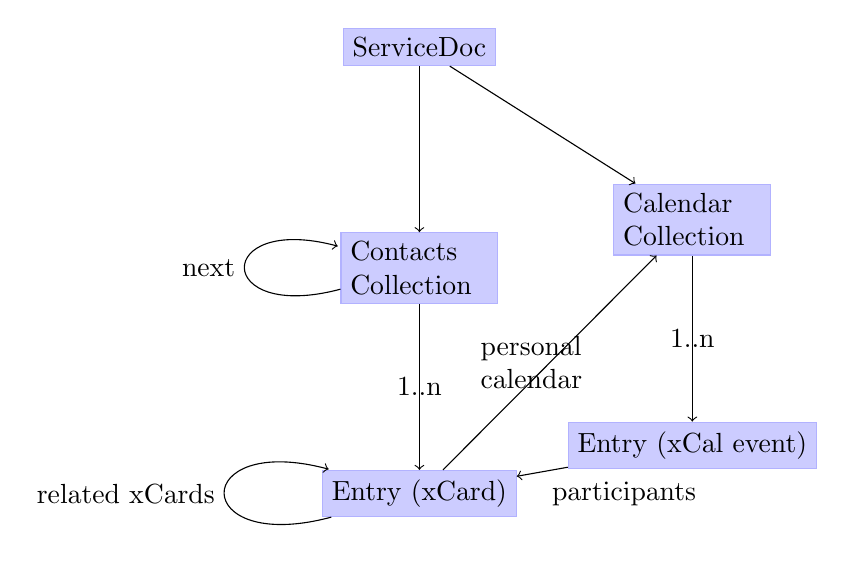
\begin{tikzpicture}
    [doc/.style={rectangle,draw=blue!30,fill=blue!20, node distance=6em}]
    \node[doc] (svc) [] {ServiceDoc};
    \node[doc] (collect) [below=of svc,text width=5em] {Contacts Collection}
      edge [<-] node {} (svc)
      edge [->, loop left] node {next} (collect);

    \node[doc] (calcollect) [below right=of svc,text width=5em] {Calendar Collection}
      edge [<-] node {} (svc);

    \node[doc] (entry) [below=of collect] {Entry (xCard)}
      edge [<-] node {1..n} (collect)
      edge [->] node [text width=5em] {personal calendar} (calcollect)
      edge [->, loop left] node {related xCards} (entry);

    \node[doc] (event) [below=of calcollect] {Entry (xCal event)}
      edge [<-] node {1..n} (calcollect)
      edge [->] node [below right] {participants} (entry);


  \end{tikzpicture}
  \caption{Discovery paths from the Service Document to individual Groupware Resources}
\end{figure}

\subsection{Efficient Synchronization with HTTP Delta encoding}
\label{sec:effic-synchr-with}

The synchronization method described in \autoref{sec:synchr-coll} can be
enhanced to reduce the bandwidth usage and general resource usage of both client
and server. The necessary extension has been described in \cite{Wyman2004} and
is commonly referred to as RFC3229+Feed since it adds a feed specific Instance
Method (IM) to the ``Delta encoding in HTTP''
standard\cite{RFC3229}. Unfortunately nobody has yet invested the effort to
drive this method through a formal standardization
process\footnote{\citeurl{http://bob.wyman.us/main/2006/04/microsoft_to_su.html}{2012-3-9}}. It
is however reported to be widely
implemented\footnote{\citeurl{http://www.wyman.us/main/2004/09/implementations.html}{2012-1-6}},
even in the popular Microsoft Internet
Explorer\footnote{\citeurl{http://blogs.msdn.com/b/rssteam/archive/2006/04/08/571509.aspx}{2012-3-9}}
and the author claims substantial bandwidths saving opportunities
\footnote{\citeurl{http://wyman.us/main/2004/10/massive_bandwid.html}{2012-3-9}}.

The idea of delta encoding is that a server can respond to conditional GET
requests with only a small, special patch. The client applies the patch to its
cached representation of the requested resource which results in the new version
of the resource. All currently IANA registered IMs are byte
oriented\footnote{\citeurl{http://www.iana.org/assignments/inst-man-values/inst-man-values.xml}{2012-3-9}}. These
methods however don't add substantial benefit for the case of synchronization
feeds.\footnote{Byte oriented IMs might however be very beneficial to serve
  updates of xCard/xCal resources if only one or a few fields changed.}

In the case of the proposed feed IM, the client sends a conditional GET to
request the synchronization feed but indicates in the ``A-IM'' header that it
understands the feed IM:
\begin{lstlisting}
GET /api/collections/contacts HTTP/1.1
Host: bar.example.net
If-None-Match: "3631-@2147483647"
A-IM: feed, gzip
\end{lstlisting}
The server responds with a valid feed including the normal head elements but can
use the etag from the ``If-None-Match'' header to include only those entries in
the response, that have changed since the time when the etag was valid. This
implies of course, that the server is able to match the given etag to a
corresponding list of changes\footnote{The given example already suggests that
  the etag itself could include database ids or timestamps.}. The server
response uses HTTP code ``226 IM Used''\cite{RFC3229} to mark the response as a
special one that is not the regular, cachaable representation.

It is advisable to also include a ``next'' link to the subsequent feed to keep
compatibility with the synchronization process from \autoref{sec:synchr-coll}
and prevent the client from accidentally considering the returned feed to
contain the full collection. The ``next'' link however would probably cause the
client to unnecessarily follow it, since it has not yet seen an entry with an
old enough ``app:edited'' value. The server could include additional entries
from its database to satisfy the client's terminating condition. Or the server
could include an artificial, minimal
deleted-entry\cite{draft-snell-atompub-tombstones-14} tag with a non-existent
ref value and a when value just older then the etag sent by the client:
\begin{lstlisting}
<at:deleted-entry
   xmlns:at="http://purl.org/atompub/tombstones/1.0"
   ref="tag:example.org,2005:NONEXISTENT"
   when="2005-11-29T12:11:12Z"/>
\end{lstlisting}
The above precautions not to break the client's synchronization logic is
necessary to permit the server to also respond to RFC3229+Feed requests with
paginated feeds in cases where more entries have changed then the server is
comfortable to include in a single response.

\subsection{Media Entries and the content tag}
\label{sec:inline-feeds-or}

The Atom format provides the opportunity to include a full representation of a
resource in the content tag of an entry\cite[sec. 4.1.3]{RFC4287}. It is thus
possible to embed complete xCard or xCal resources in the Atom feed
and so to relieve the client from issuing many GET requests for each individual
resource.

The benefit of saved GET requests must be balanced with the possible
disadvantage of serving the client resource representations already seen. A
client that does regular updates may probably be interested only in the first
one or two entries of a feed while the server might have made the effort to
produce tens of entries.

On the other hand the Atom Format mandates that an entry without embedded
content must provide a summary element. It may not make much of a difference in
bandwidth and processing whether a summary is produced or the full content is
provided.

Different optimization strategies are possible here, e.g.

\begin{itemize}
\item The first feed in a sequence of paged feeds could contain only very few
  entries to optimize for regular updates and have more entries in all following
  feeds.
\item The server could remember the entries already consumed by an authenticated
  client and serve only new entries in the first feed.
\end{itemize}

In any case it is mandatory that a client can handle embedded content as well as
linked content.

\subsection{Modifying Resources and Offline editing}

Editing, Updating and Deleting of media entries is specified in the Atom
Publishing Protocol and is useful for this work without modifications.

% As outlined in \autoref{sec:inline-feeds-or} it is possible to include full
% representations of the collection resources in the content tag of an entry. A
% client however is not allowed to use an embedded resource representation as the
% base for an update\cite[sec. 10]{RFC5023}. If the client has not yet retrieved
% the resource from its own URI it thus `` SHOULD perform a GET on the URI of the
% Member Entry before editing it.''[Ibid.] This limitation is consequent since the
% Atom feed does not contain an ETag for an embedded resource. A client thus can
% not make a conditional PUT request only from the information in the
% feed.\footnote{Google adds an etag attribute to the entry tag in its data
%   api. \citeurl{http://code.google.com/apis/gdata/docs/2.0/reference.html\#ResourceVersioning}{2012-2-13}}

In addition to the normal online workflow, a client should offer the user the
possibility to create, update and delete resources while being offline and to
apply this modifications during the next synchronization, much like the IMAP
protocol used by Kolab. This requirement is trivial to fulfill as long as no
concurrent edits happen on the server site. In that case the client just PUTs
the changes the next time it is connected.

In the case of edit conflicts however, the client needs to perform an automated
or user assisted merge of the conflicting resources. Therefor the client should
always preserve a copy of a resource version as last seen from the Server to be
able to perform a three-way-merge.

The problem of offline edits and conflicts is thus similar to the case of a
failed conditional PUT request due to a concurrent edit. \cite{Nielsen1999}
describes this case and resolutions in detail.


\subsection{Special Reports, Queries, Search}
\label{sec:spec-reports-search}

In few cases it may not be feasible for a client to synchronize a full
collection, e.g. due to low bandwidth. This section explores restful ways to let
the client request only a subset (selection) of a collection. More specifically
the client should be informed about possible query facilities without relying on
out-of-band information.

A promising approach is to use the de-facto standard
OpenSearch\cite{Clinton}. According to its homepage it is implemented by most
major browsers, search engines and many other sites. OpenSearch is also
recommended for the link type ``search'' in the HTML5
standard\cite[sec. 4.12.4.12]{Hickson2011a}. The default format of an OpenSearch
result list is an Atom (or RSS) feed.

OpenSearch defines the (not yet IANA registered) media type
application/opensearchdescription+xml, which provides necessary information for
a client to perform queries against a search service. Since possible search
queries are usually unlimited it is not possible anymore to provide a set of
static links. Instead the server provides an ``URI Template''\cite{RFC6570}
that instructs the client how to perform an ``URI
construction''\footnote{OpenSearch is the older standard and referenced as Level
  1 URI Templates in \cite{RFC6570}.}.

The basic OpenSearch standard defines a simple full text search. Thus a user
could search contacts by name, address or any other field value. Equally events,
todo items or notes could be searched by keywords.

The next important use case is to show calendar events in a given interval,
e.g. to present the events for a month, week or day. This can be achieved with
the OpenSearch Time extension that provides the temporal start and end
parameters. Rob Yates CalAtom\cite{draft-yates-atompub-calatom-00.txt} proposal
included a similar time range search as the only but mandatory special report.

Probably useful might be the OpenSocial Geo extension. It could allow to search
contacts or events in a given geographic region. Even more search types become
possible with the SRU extension that wraps the ``Search/Retrieval via URL''
standard with its ``Contextual Query Language''
(CQL)\footnote{\citeurl{http://www.loc.gov/standards/sru}{2012-3-1}}. The latter
provides the possibility to sort result sets which might be interesting to
present an address book sorted by names.

Search result Atom feeds can make use of annotated HTML
(\autoref{sec:microdata}) in the summaries of entries and should not embed full
resources in the content tag. Thus the client can still provide a structured
view of the data, like calendar views or a tabular contacts list without the
need to transfer full representations.

The OpenSearch specification suggests that links to the OpenSearch Description
Document for an Atom feed might be added inside a feed tag. There is however no
reason not to add such a link inside the collection tag of a Service
Document. This allows a client to directly search a collection without the need
to get the feed first.

% \subsubsection{Structural and Behavioral Rest Model}
% @TODO Modelierung der Anwendung mit dem Meta Model nach Schreier.
% Primary Resources: Contacts, Calendars, ...
% List Resources: 


% http://lists.calconnect.org/pipermail/caldeveloper-l/2012-March/000177.html
% "The only queries I have seen clients doing are time-range ones."
% Cyrus Daboo

\section{Other Design Considerations}
\label{sec:design}

% > - Es wird gezeigt, dass AtomPub mit ein paar, meist bereits standardisierten
% >   Ergänzungen eine sinnvolle, resourcenorientierte Alternative zu C.*DAV,
% >   OpenSocial ist.

% > - Diskussion der Problematik, dass viele Medientypen in XML definiert sind, 
% > aber
% >   viele Webentwickler JSON bevorzugen. Eine automatisierte Übersetzung von XML
% >   Schemas in JSON Schemas ist nicht möglich, also muss für alle XML 
% > Medientypen
% >   eine JSON Äquivalent manuel definiert werden.

% > - Darstellung semantically annotated HTML mit drei verschiedenen Formaten,
% >   Begründung der Formatauswahl. Vorschlag zur Implementierung mit einer
% >   Templateengine und automatisierten Erstellung der Microdata Strukturelemente

% > - HTML Forms und ihre Einbettung in eine Hypermedia API:
% >   - Kein PUT/DELETE
% >   - universeller, nichtssagender Medientyp application/x-www-form-urlencoded
% >   - keine link-relation, um auf die Form zur Erstellung einer neuen Resource 
% > zu
% >     verweisen.

% > - Problematik des Updates mit nicht isomorphen Medientypen, Möglichkeiten, 
% > damit umzugehen


\subsection{Media Type conversion and non-isomorphism}

Two media types are non isomorphic, if at least one of them can express
information which the other could not express. For example the vcard media type
defines many property parameters that have no equivalent in portable contacts,
like language, altid or sort-as. So a conversion of a vcard into portable
contacts will most likely lose this data.

This data loss could first be a problem when a client receives a
representation. However since the client negotiated the media type with the
server it is most likely that it is satisfied with only the data representable
in that data type.

Now if the client uses such a media type in a put request to update a resource,
it may not be clear how to deal with the information the client could not
express in the submitted resource. Should it be deleted or merged with the new
representation?

Different strategies are possible in such scenarios and must be selected for the
individual use case:

\begin{enumerate}
\item The server accepts updates only for one media type while serving other
  media types in a ``read-only'' mode.
\item The server accepts PATCH requests\cite{RFC5789} as a compromise while
  still not accepting certain media types for updates
  (\autoref{sec:patching-resources}).
\item The implementer decides to either merge or deletes information not
  representable in a received media type and lives with the consequences. In the
  case of contact information this can be a valid strategy since the most
  essential information is representable in all media types. The server
  practically only works with data in the intersection of all supported media
  types.
\item Available facilities to extend media types are used to establish
  isomorphism. Vcard for example allows the addition of arbitrary properties
  prefixed with ``x-''.
\item The server implements version control so that the situation can be
  resolved manually later.
\end{enumerate}

The creation of resources can be handled more liberate then updating, since no
state on the server exists that could be lost.


\subsection{Microformats, Microdata, RDFa}
\label{sec:microdata}
%TODO Schreier:nach dem lesen des einführenden Abschnitts weiss der Leser nicht, was er im Rest des Abschnitts zu erwarten hat, dementsprechend ist die Motivation für die Abschnitte unklar und es fällt schwer den roten Faden zu finden

HTML documents are primarily meant to be rendered by browsers and interpreted by
humans. It is hard for a machine to interpret the meaning of text and data
included in an HTML document. To help this, different techniques have evolved to
add additional meta data to HTML that allows machines to identify structured
data in HTML without having an impact on the rendering. The most popular ones,
Microformats, Microdata and RDFa, are presented and discussed in
\cite{Tennison2012}.

There is not yet an established term to refer to the three different
formats. Practitioners use ``structured data languages''\cite{Sporny2011},
``machine-readable data format''\cite{Hickson2011}, ``structured data
markup''\cite{Goel2011} or just ``structured markup''. Scientific publications
seem to use the term ``Semantic annotation''\cite{instance7} to refer to HTML
with machine readable semantic data. This work will use the term ``Semantic
annotation format'' to refer to Microformats, Microdata, RDFa and similar
formats.

\subsubsection{Use Cases}
\label{sec:semantic-anno-use-cases}

One major use case for semantic annotations is to help search engines to better
index the annotated site. The Microformats project was started by a blog search
engine (Technorati)\cite{Celik2006} and the recent schema.org effort came from
the three big search engines Google, Bing and Yahoo.\cite{Goel2011} Another use
case is demonstrated by the Firefox plugin
``Operator''.\footnote{\citeurl{https://addons.mozilla.org/en-US/firefox/addon/operator/}{2012-2-20}}
It allows to extract annotated entities from web pages. A user could thus import
contact or event data from arbitrary web pages in his personal information
manager with one click. Semantic annotations can also be used to make web
content accessible to disabled people\cite{Yesilada:2007:EDS:1279700.1279704}.

A third use case is currently under development as part of the European Union
Research Project ``Interactive Knowledge Stack'' (IKS) that builds a semantic
content management stack. The sub-project ``Vienna IKS Editables''
(VIE)\footnote{\citeurl{http://www.iks-project.eu/projects/vienna-iks-editables}{2012-2-20}}
uses semantic annotations to make content on a web site editable. It does so by
searching the HTML document for semantically annotated entities and dynamically
building editing interfaces for those. A modified entity can then be sent to the
server via AJAX in a format called ``json-ld'' that serializes semantic data to
JSON.\footnote{\citeurl{http://json-ld.org}{2012-2-20} the iana registration of
  the mime type \lstinline:application/ld+json: is currently discussed}
For a Groupware, this editor could be used to automatically create HTML forms instead
of creating them on the server site.

\begin{anylisting}[label=fig:microdata-atom-summary,
                   language=xml,
                   caption={Microdata used in the summary of an ATOM entry summary (markup not escaped for clarity)}]
<summary type="html">
  <div itemscope itemtype="http://schema.org/Person">
    <a itemprop="url" href="www.maxpattern.name">
      <div itemprop="name"><strong>
        <span itemprop="givenName">Max</span>
        <span itemprop="familyName">Pattern</span>
      </strong></div>
    </a>
    <div itemscope
         itemtype="http://schema.org/Organization">
      <span itemprop="name">
        Andorian Mining Cooperation
      </span>
    </div>
    <div itemprop="email">some@mail.com</div>
    <div>
      <meta itemprop="birthDate" content="1970-01-02">
      DOB: 01/02/1970
    </div>
  </div>
</summary>  
\end{anylisting}

In the context of this work, semantic annotations could be used inside the
\lstinline:summary: tag of Atom entries, as shown in listing
\ref{fig:microdata-atom-summary}. A consumer of a feed of contact elements could
thus use the data extracted from the annotated summary data to provide a tabular
overview of the entries even without fetching the associated media resource of
the entry, which is especially useful for search results as discussed in
\autoref{sec:spec-reports-search}.

\subsubsection{Format selection}

With at least three different semantic annotation formats, a developer needs to
decide which to implement. It is possible to implement multiple formats in
parallel inside the same HTML document, but this means more markup and a more
complex publishing task\cite{Tennison2012}. This choice is not a choice of
different Media Types, but a choice in the scope of the Media Type text/html (or
application/xhtml+xml).

A first consideration has to be the ability of expected consumers to handle the
format, a second consideration the available tooling to produce a particular
format. The different Semantic annotation formats impose certain requirements
for the used HTML dialect. Microformats can be used with all versions of HTML,
RDFa with XHTML or HTML5 and Microdata introduces special attributes that work
only with HTML5\cite{Tennison2012}.

Microdata is part of HTML5 and a standard effort of the W3C\cite{Hickson2011}.
It is also backed up by the schema.org effort of Google and
Microsoft.\footnote{\citeurl{http://schema.org/docs/gs.html\#microdata_why}{2012-2-17}}
The schema.org vocabulary in turn has been mapped to the semantic world by
researchers working on linked
data.\footnote{\citeurl{http://schema.rdfs.org/about.html}{2012-2-17}} Thus by
using Microdata with the schema.org vocabulary, the data can easily be combined
with other semantic data. The rest of this work therefor concentrates on
Microdata. Many good arguments to also consider RDFa can be found in the blog of
Manu
Sporny\footnote{\citeurl{http://manu.sporny.org/category/rdfa/}{2012-2-20}},
chair of the RDF Web Applications Working Group at the World Wide Web
Consortium.

% detailed pro cons microdata vs. RFDa http://www.jenitennison.com/blog/node/165

\subsection{HTML Forms}
\label{sec:html-forms}
%@TODO
TODO

A web based user interface for a Groupware today has many means to provide data
editing and submission facilities thanks to powerful Javascript libraries like
the VIE Editor (\autoref{sec:semantic-anno-use-cases}). The traditional,
standardized and most compatible way however is the use of HTML forms. These
however lack a few features that could improve their use for restful systems.

HTML has no means to send an etag when submitting a form and no support for
other HTTP verbs then GET and POST, most importantly PUT and DELETE. A
Discussion to include these however seems to be underway\cite{Amundsen2011}.

All forms have the same media type of application/x-www-form-urlencoded,
although they may represent totally different kind of resources. In practice
this is often not a problem since the server knows which form to expect and
selects its parsing routine accordingly.

In cases, where different forms can be expected to be submitted to the same URI,
e.g. to the URI of a collection, the server needs to be informed about the
resource type, probably by a hidden form input element.

The manual creation of HTML forms and associated form parsers and validators is
involved and error prone. Therefor many approaches and implementations exist to
automate this task. If a machine can work on an existing data model for the
resource, then this can be used as basis for the automation.

TODO: Means to automatically build forms from descriptions of the data:
``Dynamic Object Model'' (Dirk Riehle) or ``Adaptive Object-Model'' (Yoder,
Johnson) implemented e.g. by eZPublish, Drupal
%@TODO
% automatically build forms like eZPublish / Drupal?

Not yet answered is the question, where or under which condition an HTML form
should be submitted to the user. It is certainly not desirable to present HTML
forms by default in every HTML representation of any resource that the user is
authorized to modify. And even then, there would still not be any mean for the
user to reach an HTML form to create a new resource.

The edit case can be solved with the IANA registered ``edit'' link-relation. An
HTML page representing an editable resource could just use a link element for
the purpose of signaling the client the location where it can retrieve an
editable resource:

\begin{lstlisting}{language=xml}
  <link rel="edit" href="?edit=true"/>
\end{lstlisting}

The above link is a relative Link that just appends a query part to the URI of
the current page (assuming that the page URI does not already contain a query
part).

It may be noted here, that making different representations of one resource
available under different URIs is no violation of rest principles and even
encouraged for similar use cases by \cite{Raman2006}.

Unfortunately no link relation is standardized to retrieve an empty form for the
creation of a new resource.\footnote{The \lstinline:Collection+JSON: Mediatype solves this issue by providing templates for new items inside the collection representation (\autoref{sec:collection+json}).}
 So for the time being server and client would need
to agree on a custom link relation for that purpose. The empty form can be
regarded as an entity of its own, linked from the collection where newly created
resources are expected to appear.

\section{Implementation}
\label{sec:implementation}


\subsection{Control Flow Overview}
\label{sec:overview}

\autoref{fig:executionflowoverview} outlines the most important classes for the
control flow. The implementation relies on the JAX-RS\cite{JAX-RS1.1}
implementation Jersey to route calls to the four different ``Jersey Resources''
classes, representing Atom Service Documents, Atom Collections, Atom Entries and
Media Resources of different Mediatypes.

The Jersey Reader/Writer providers are called by Jersey to transform in- and
output for the Resource classes. The \lstinline:AbderaWriterJerseyProvider: just
uses the Abdera library. The other two providers are special because they work
on the universal \lstinline:Resource: class or the related
\lstinline:UnparsedResource: class. These classes represent the concept of
resources that can be represented with different Mediatypes. They are discussed
in detail in \autoref{sec:resource-handling}.

One instance of the CollectionStorage interface is responsible for the
administration of one collection of Resources. The first four methods implement
CRUD functionality and the \lstinline:listUpdates: method provides a partial,
time ordered list of updated resources, including special Resources to indicate
deletions. This list can be directly transformed in a corresponding AtomPub
feed.

Like the other classes, the CollectionStorage deals with the universal
\lstinline:Resource: class. The Precond(itions) parameter is a wrapper class
around the corresponding HTTP headers\footnote{If-Match, If-None-Match,
  If-Modified-Since, If-Unmodified-Since}. It provides
\lstinline:shouldPerform(etag, updated):bool: methods that the storage must call
with the resource's etag, last update timestamp or both. The CollectionStorage
indicates with each methods return value, whether it actually performed any
action. The GetResult and ResultList classes are simple tuple classes wrapping
one or multiple \lstinline:Resource: instances in case the Preconditions failed
or otherwise an indication that a ``304 Not Modified'' response should be
returned.

\begin{figure}[htb]
  \centering
  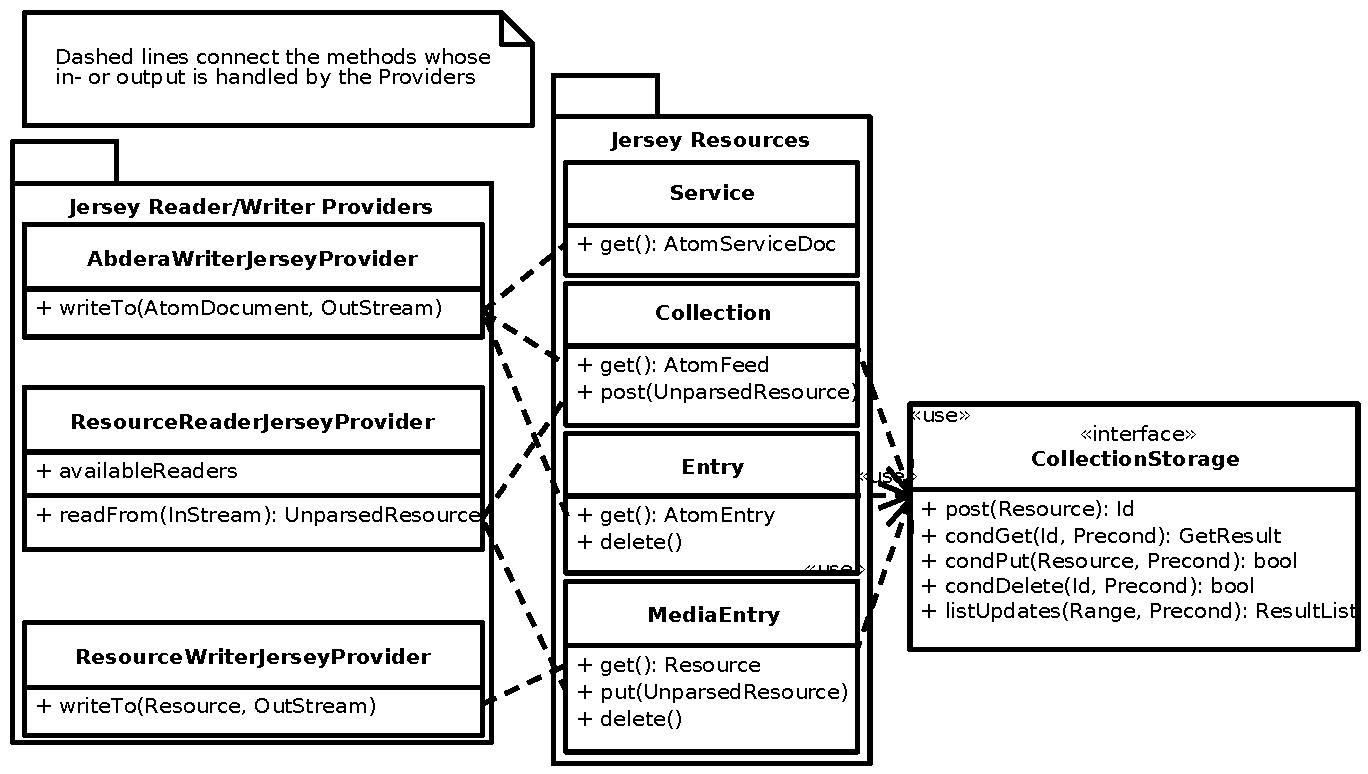
\includegraphics[width=1.2\textwidth]{executionflowoverview}

  \caption{Overview of the control flow}
  \label{fig:executionflowoverview}
\end{figure}

\subsection{Resource handling}
\label{sec:resource-handling}
% Resource Klasse

% Komplexität der Behandlung verschiedener Medientypen versteckt hinter
% "Resource" Klasse mit Hilfe von ResourceFacades

% Die Mächtigkeit der Resourceklasse ermöglicht dass der restliche Code,
% z.B. CollectionStorage sehr einfach gehalten werden kann.

The \lstinline:Resource: class is the generalization of a restful HTTP resource
without a binding to a specific Mediatype. This corresponds to the distinction
between a resource and its representations in Fielding's
Dissertation\cite[sec. 5.2.1.1]{Fielding2000}. A representation in a certain
format is a property ``selected dynamically based on the capabilities or desires of
the recipient and the nature of the
resource''\cite[p. 87]{Fielding2000}.

\subsubsection{Resource properties}
\label{sec:resource-properties}

The interface of the \lstinline:Resource: class marks the border between code
that handles the control flow of an HTTP request, as outlined in
\autoref{fig:executionflowoverview}, and code that provides information about
properties of a resource (\autoref{sec:resourcefacades}). In the context of this
work, four different kind of properties of resources are distinguished:

\begin{itemize}
\item essential administration properties: unique Id, last update time, HTTP
  entity tag
\item generic meta properties: title, summary, author
\item a Mediatype independent interface corresponding to the concept represented
  by the resource e.g., a person, location, event, product, \ldots
\item a mediatype specific serialization (representation) of the resource
\end{itemize}

The id and update time are required for the synchronization protocol outlined in
\autoref{sec:interactions}. They do not depend of the nature or content of the
resource and are attached to the resource by code outside of the
\lstinline:Resource: class. The entity tag must differ for each new version of a
resource. The code to produce and check a resource's entity tag should be
adjusted carefully with the concrete CollectionStorage implementation to ensure
efficient processing of conditional HTTP requests.

The generic meta properties of the resource can be used to fill the
corresponding tags of an atom entry. They can either be extracted from a
meaningful property of the resource or be provided to the resource. E.g., the
author property could be extracted from the meta data of an image file (EXIF),
set to the organizer of an ical event. The title of a contact resource in the
implementation is set to its full name and email. The summary also contains the
address and phone number.

One use of two mediatype independent interfaces or ``facades'' or a resource is
exemplified in \autoref{fig:titleandsummary}. The \lstinline:Contact: interface
is implemented by two classes that can extract the necessary information from
either a \lstinline:VCard: or a \lstinline:PortableContact: instance. The
\lstinline:Contact: interface in turn is used by an implementation of the
\lstinline:TitleAndSummary: interface. The \lstinline:PlainTextTitleAndSummary:
class in comparison does not work on an intermediary interface but directly on
the original data structure.

The above mechanism is exposed by the \lstinline:getFacade(Interface): method of
the \lstinline:Resource: class and used to retrieve a
\lstinline:TitleAndSummary: facade in order to build an Atom Entry. The code
using the facade does not need any further knowledge about the type of resource
it is working with.

\begin{figure}[htb]
  \centering
  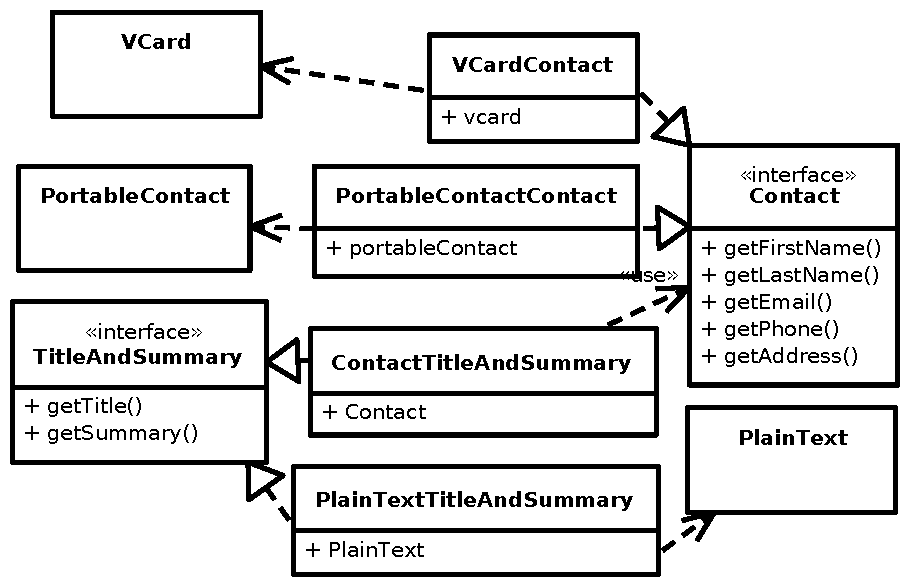
\includegraphics[width=1\textwidth]{titleandsummary}

  \caption{Dependency of facades of resources to provide the TitleAndSummary interface}
  \label{fig:titleandsummary}
\end{figure}

The serialization property is exposed by the asMediaType(MediaType,
OutputStream) method of the \lstinline:Resource: class. Internally this method
also uses the \lstinline:getFacade(): mechanism to requests an instance of a
\lstinline:Writer: interface with the additional constraint that the writer must
produce the requested Mediatype (\autoref{sec:resourcefacades}). Accordingly the
\lstinline:ResourceWriterJerseyProvider: of \autoref{fig:executionflowoverview}
is trivially simple: It just calls the asMediaType method of the provided
resource. The Resource is responsible for providing a mediatype specific
representation of itself.

The Resource class outlined in this section does not correspond to the equally
named resource class concept in JAX-RS\cite{JAX-RS1.1}. The JAX-RS resource
classes in this work are found in the ``Jersey Resources'' package of
\autoref{fig:executionflowoverview}. But they do not really represent resources
but rather the binding of resources to URIs and their processing logic.

\subsubsection{Resource life cycle}
\label{sec:resource-life-cycle}

Resource classes in this work have a four staged life cycle.  The first stage is
represented by the \lstinline:UnparsedResource: class, instantiated by the
ResourceReaderJerseyProvider class for post or put requests. In this stage the
Resource has already been assigned an appropriate \lstinline:Reader:
implementation according to the Content-Type request header but it has not yet
received an Id and update timestamp.

The \lstinline:Resource: class represents the second stage, a parsed request
body with an Id and update timestamp. Only in this stage the getFacade() method
can be used.

Once a resource has been deleted, it does not vanish entirely, but enters stage
three. Only the associated data originally submitted in the request body is
discarded but the Id and update timestamp (now referring to the time of
deletion) is preserved. Such a ``deleted resource'' is used to generate the
``deleted-entry'' entries in the AtomPub feed (\autoref{sec:synchr-coll}).

Deleted resources don't need to be preserved eternally. A deleted resource with
the oldest timestamp of all resources managed by a particular CollectionStorage
can be safely purged completely (stage four). A client that synchronizes the
collection can still infer that the resource has been deleted since it is no
longer included anywhere in the list of updates. Repeated application of the
above rule makes sure that the last element of the updates list points to a
``living'' Resource of the second stage.

\subsubsection{Resource Facades}
\label{sec:resourcefacades}

\autoref{sec:resource-properties} introduced and motivated the concept of
Resource Facades. This section explains the inner workings of the classes
providing this mechanism as drafted in \autoref{fig:resourcefacades}.

The Resource class does not hold any attribute that directly corresponds to its
``main data''. Instead it holds a FacadeProvider instance to request a specific
data facade to access data. Facades are primarily referenced by Java interfaces.

A FacadeProvider in turn is instantiated with a FacadeRegistry of available
FacadeFactories and one or more ``seed'' facades, making up the initial content
of the resolvedFacades attribute. An instance of FacadeFactory is capable of
building one specific facade object and has a set of dependencies needed for
that purpose. Therefor the concrete FacadeFactory used to build a facade and
thus the resulting implementation of the facade interface depends on the facades
already available in the resolvedFacades attribute of the FacadeProvider.

In the example of \autoref{fig:titleandsummary}, the TitleAndSummary interface
is implemented by two different classes. The factory responsible for the
PlainTextTitleAndSummary would declare a dependency on a PlainText facade. The
factory producing the ContactTitleAndSummary declares a dependency on a Contact
facade, which can again be produced by two different factories with their
dependencies finally pointing to the ``root'' facades.

Facades already resolved are added to the resolvedFacades attribute of the
FacadeProvider to speed up future facade requests. This is possible since
facades are required to only provide read access to the data. Any manipulation
of the Resource should result in a new Resource instance thus reflecting the
REST characteristic that Resources are manipulated by the submission of new
Representations.

Requests for facades can be further parameterized with a Predicate. The
Predicate has one apply(FacadeFactory):bool method which is called only for
FacadeFactories producing the desired interface. This mechanism is used in the
implementation to check an \lstinline:isWriteable(MediaType): method on
factories producing Writer instances and thus to select the correct Writer
according to the Mediatype accepted by the client. Future work could
considerably enhance this rather brittle mechanism e.g., to check for
annotations on the class produced by the factory.

\begin{figure}[htb]
  \centering
  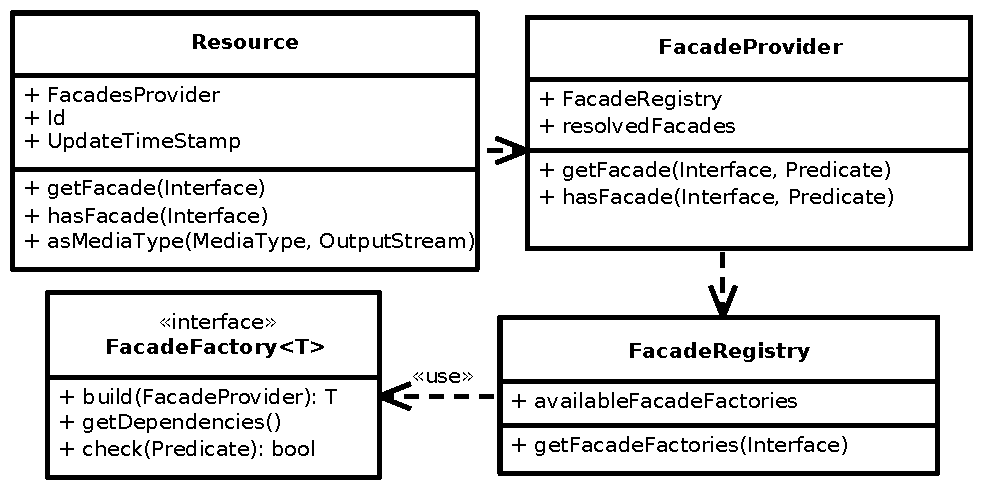
\includegraphics[width=1\textwidth]{resourcefacades}

  \caption{The API of the Resource Facades mechanism}
  \label{fig:resourcefacades}
\end{figure}

The Resource Facades concept is implemented only as a proof of
concept. \autoref{sec:resourcefacadesfuture-work} outlines a lot of future work
that might be worth of consideration in this direction.

% A resource method should contain the programming logic executed to serve a
% request of a specific type (e.g. GET, PUT) against a specific resource. The
% programming logic could execute common tasks like the following:

% \begin{itemize}
% \item validate the correctness of a submitted resource
% \item check the clients authorization
% \item persist the submitted resource data
% \item trigger notifications containing a summary of the resource
% \item submit the submitted resource to an indexing system
% \item check the submitted resource to be of a certain accepted domain type, like
%   contact, event, todo item or any set of such types
% \end{itemize}

% All the above processing tasks should in theory be independent of the media type
% of a resource and only be programmed once to work on any resource format. This
% could be made possible by applying the concept of roles to resources. Roles have
% been described already 15 years ago by \cite{Fowler1997} or a bit later by
% \cite{Baeumer2000}. However no evidence could be found whether roles have been
% used to implement restful systems.

% According to \cite{Steimann2008}, there exists several definitions for roles
% which mostly share a few core properties:

% \begin{quote}
%   This includes the property that a single object can play several roles of
%   different or the same kind both simultaneously and sequentially, and that the
%   same role can be played by different objects of the same and different
%   kinds. Raised to the type level, this means that the relationship between role
%   types and class types (as sources of role players) is generally m:n.
% \end{quote}

% A popular example for roles is a person, that can have the different roles over
% their lifetime (student, professor, single, husband, widower) or in different
% contexts (teacher, father, husband, customer, politician).

% \cite{Steimann2001} repeats the necessity of the dynamic role concept and argues
% that (Java) interfaces serve as an appropriate mean to handle roles.

% Exemplified with the above tasks, a resource can have the role of being
% validated, persisted, summarized or checked for being of a certain type. So like
% in the above quote a facility is needed that can provide m different roles of
% resources that come in n different shapes.

% It can be noted, that unlike in the previous example with roles of a person,
% this resource roles examples do not extend the original resource with new
% attributes. A person surely gets additional attributes as a father (references
% to children) or professor (member of faculty). Thus the term ``facade'' in favor
% of role should indicate that only different views of the same data are provided.

% Listing \ref{fig:datafacades-api} shows interfaces of a minimal framework to
% provide Facades for Resources. The idea is, that any code that needs information
% from a Resource requests the appropriate Facade from the ResourceHandler. The
% ResourceHandler was instantiated with a FacadeRegistry from which it can request
% Factories for requested Facades. A ResourceHandler must have been instantiated
% with at least one initial input Facade, e.g. an InputStream.



    % Facades provide read-only access to the data
    % Facades can depend on other Facades and thus reuse work
    % Facades could do:
    %     Parse the InputStream with a common JSON/XML framework
    %     Could check whether the data represents a concept like a contact or calendar item, independent from the underlying Media Type (vCard, xCard, portable contacts, iCal, xCal)
    %     Could provide a transformation to another representation (XML<->JSON, xCard to portable contacts)
    %     could extract generic informations from different media types: Title, Authors, Updated, Summary
    % A Facade (Java Interface) that provides access to the Name of a Contact Resource could be implemented by different classes that could work either on vCard, xCard or Portable Contacts. The resource method does not need to be aware or the original media type of the data.

% The concept is powerful because Facades can easily be added without changing
% existing classes. In JAX-RS the resource Method needs to decide, on which
% representation of the data it wants to work. With this concept, a resource
% method could use several different available Facades to access the data.

% Using a similar concept to build representations (request Facades) for different MediaTypes may not be worth the effort.
% This would mostly be necessary to handle GET requests. GET requests however are expected to be idempotent and therefor should contain little to no internal side effects.
% It therefor seems to be reasonable to provide one GET request method for every produced Media Type.
% Specialized get requests may also execute faster than an approach that needs to dynamically build the processing pipeline.

% JAF + REST proposed in 2007 http://www.javaworld.com/javaworld/jw-10-2007/jw-10-resteasy.html





\subsection{CollectionStorage}
\label{sec:collectionstorage}

The CollectionStorage interface\footnote{The interface may be further broken
  down in a read-only and a write part which has been avoided for this
  overview.} is intended to be implementable for a variety of persistency
providers like relational databases, the file system, document databases like
CouchDB, MongoDB, eXist. In this context the IMAP folders used by Kolab are just
a kind of document store.

A CollectionStorage is instantiated with the knowledge of the collection for
which it is responsible. Each collection managed by the application corresponds
to a separate CollectionStorage instance. Several CollectionStorage instances
might however share the same underlying connection to a persistency provider.

The only uncommon requirement for the persistency provider is to provide the
time ordered list of updates. This list could be thought of as just another kind
of search or report like the full text and time range search defined by
OpenSearch (\autoref{sec:spec-reports-search}). A search index library like
Apache Lucene\footnote{\citeurl{http://lucene.apache.org}{2012-03-26}} can
provide indexes for full text search on text fields, time range on events or a
list of all documents ordered by an ``updated'' field.

The IMAP based persistency of Kolab does not provide the described
indexes\footnote{The IMAP SEARCH command\cite[sec 6.4.4]{RFC3501} searches only
  the message body and headers but not attachments.}. Those must therefor be
implemented by a separate component.

To make implementation of the interface easy and to correspond to the REST
characteristic that every request is atomic, 

The CollectionStorage does not expose any support for transactions. This should
make the interface easier to implement and also corresponds to the REST
characteristics of statelessness and transfer of full representations. As a
consequence, the check for HTTP preconditions must be made inside the
CollectionStorage. Otherwise an update could be lost as demonstrated in Listing
\ref{fig:evaluatepreconditions-concurrency} from the JAX-RS
specification\cite[p. 28]{JAX-RS1.1}. In this example a concurrent update by a
separate HTTP request that would happen between the etag check and the
\lstinline:doUpdate: call would be overwritten.

\begin{javalisting}[label=fig:evaluatepreconditions-concurrency,
                   caption={Potential lost-update problem with JAX-RS}]
ResponseBuilder rb = request.evaluatePreconditions(etag);
if (rb == null)
  return doUpdate(foo);
\end{javalisting}

% @TODO a resource should not be build, it the etag has not changed. How to make
% etag checking as cheap as possible?

% Contactzilla.com saves portablecontacts json in MongoDB
% https://groups.google.com/d/msg/portablecontacts/57R9gGyoqt0/-P0fF4zRjaoJ

\subsection{Dependency Injection}
\label{sec:dependency-injection}

\subsubsection{Preparsed Request Components with Dependency Injection}
\label{sec:prep-requ-comp}

It seems like an obvious fact that could not be further deduced, that any
response action to a request must be preluded by a parsing of the request. In
the case of a REST application this parsing could be further divided in two
steps:
\begin{enumerate}
\item Parse URI, Accept Header and HTTP verb to select the Resource method
\item Resource method specific parsing as defined by annotations or done in the
  Resource method
\end{enumerate}

JAX-RS defines only rudimentary support for the second step by means of
inflexible annotations. Listing \ref{fig:jaxrs-annotated-queryparams} shows the
verbosity of parsing a set of standard query parameters for a search
interface. An alternative is shown in listing \ref{fig:request-components}. The
parsing of query parameters is delegated to the class
SearchRequest.\footnote{The QueryParams class is supposed to be an easy
  interface to access query parameters and apply rudimentary validation in one
  step.} The request method ``handleGet'' can access the parameters easily
through the injected SearchRequest instance.

\begin{javalisting}[label=fig:jaxrs-annotated-queryparams,
                   caption={Verbosity of parsing Requests with JAX-RS}]
@Get public Response get(
    @QueryParam("query") String query,
    @QueryParam("sort-by") String sortBy,
    @QueryParam("offset") int offset,
    @QueryParam("limit") int limit ) {
\end{javalisting}

\begin{javalisting}[label=fig:request-components,
                   caption={Separating Request parsing from the Resource method}]
@GET @Inject
public Response handleGet(SearchRequest sr) { ... }

@RequestScoped
public class SearchRequest {
    public final String query, sortBy;
    public final int offset, limit;
    
    @Inject public SearchRequest(QueryParams qp) {
        query = qp.getNotEmpty("query");
        sortBy = qp.getOrElse("sort-by", "score");
        offset = qp.getPositiveIntOrElse("offset", 0);
        limit = qp.getPositiveIntOrElse("limit", -1);
    }
}
\end{javalisting}

The main advantages of this approach would be:

\begin{itemize}
\item Classes parsing commonly used query parameters can be reused.
\item The request method declaration gets much easier to read.
\item Sophisticated validation can be applied without obfuscating the request method.
\item Default values for unspecified input could depend on information only
  available at runtime instead of being provided as static value to the
  applications source code.
\end{itemize}

This approach is possible to implement for example with the dependency injection
support provided by the Jersey
framework.\footnote{\citeurl{http://codahale.com/what-makes-jersey-interesting-parameter-classes/}{2012-2-5},
  \citeurl{http://codahale.com/what-makes-jersey-interesting-injection-providers/}{2012-2-5}}

\begin{figure}[tbph]
  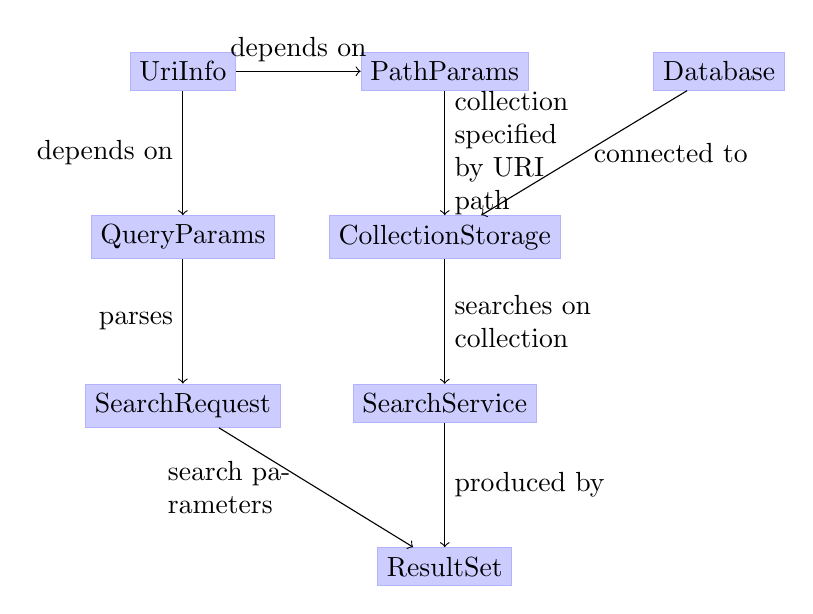
\begin{tikzpicture}
    [doc/.style={rectangle,draw=blue!30,fill=blue!20, node distance=4.5em}]

    \node[doc] (uriinfo) [] {UriInfo};
    \node[doc] (queryparams) [below=of uriinfo] {QueryParams}
      edge [<-] node [left] {depends on} (uriinfo);

    \node[doc] (searchrequest) [below=of queryparams] {SearchRequest}
      edge [<-] node [left] {parses} (queryparams);

    \node[doc] (pathparams) [right=of uriinfo] {PathParams}
      edge [<-] node [above] {depends on} (uriinfo);

    \node[doc] (database) [right=of pathparams] {Database};

    \node[doc] (collection) [below=of pathparams] {CollectionStorage}
      edge [<-] node [right] {connected to} (database)
      edge [<-] node [right,text width=5em] {collection specified by URI path} (pathparams);

    \node[doc] (searchservice) [below=of collection] {SearchService}
      edge [<-] node [right,text width=5em] {searches on collection} (collection);

    \node[doc] (resultset) [below=of searchservice] {ResultSet}
      edge [<-] node [left,text width=5em] {search parameters} (searchrequest)
      edge [<-] node [right] {produced by} (searchservice);
  \end{tikzpicture}
  \caption{Building a processing pipeline with Dependency Injection}
  \label{fig:dependency-injection-pipeline}
\end{figure}

\subsubsection{Driving Dependency Injection further}

The use of dependency injection could be extended to comprise several levels of
dependencies and thus to build processing pipelines.  The information from the
above SearchRequest class is probably just forwarded by ``handleGet'' to another
component that executes the search on a given collection. Thus the request
methot is ultimately interested on the search result set to transform it into a
response. Consequently the ``handleGet'' method could use dependency injection
to request the result set and only start working on this. Figure
\ref{fig:dependency-injection-pipeline} visualizes the hypothetic dependency
graph of an application specific ResultSet class.

The figure shows how the CollectionStorage to search on is identified by the URI
path and the search parameters by the SearchRequest class of listing
\ref{fig:request-components}. The dependency injection is configured to produce
a ResultSet class by executing a SearchService with the request scoped
CollectionStorage and SearchRequest.

The idea might be an alternative implementation of processing pipelines to the
one proposed in \cite{Davis:2011:XTR:1967428.1967437}, which uses XProc, An XML
Pipeline Language. One advantage of the dependency injection approach would be
that the processing pipeline can be defined and configured in the same language
then the rest of the application.

%@TODO
%\subsection{Client Design}
%What needs a client to know, how does it need to work?

\subsection{Producing Semantically annotated HTML}
% XML transformations with scalate http://scalate.fusesource.org/documentation/scuery.html

A recent discussion of possibilities to produce semantically annotated HTML can
be found in \cite[sec. 9.1.3]{DBLP:books/daglib/0023755}. The authors describe a
method developed as part of a larger ``Web Semantics Design Method'' (WSDM),
consists of two mappings. The first one is the ``data source mapping (DSM),
which describes exactly how the reference ontology maps to the actual data
source.''  The second mapping links HTML tags to elements of the reference
ontology from the first mapping. Neither the book nor referenced papers however
go in any more detail about the final step of generating the annotated HTML
tags.

One important point can be learned from the WSDM description. The production of
semantically annotated HTML can become a lot easier if the entity is already
available represented with the targeted vocabulary. A very naive approach to
produce annotated HTML would be to just manually write the necessary attributes
in the template and fill them with values from an arbitrary data object, as
demonstrated in listing \ref{fig:naive-microdata-template}. Even with the
conciseness of the used template language
Jade\footnote{\citeurl{http://scalate.fusesource.org/documentation/jade-syntax.html}{2012-2-22}
  Jade is the most concise among several supported template languages of the
  Scalate Template Engine.}, the developer still has a lot to type.

\begin{anylisting}[label=fig:naive-microdata-template,
                   caption={Defining all Microdata attributes manually in an HTML template}]
-@ var vcard: VCard

div( itemscope itemtype="http://schema.org/Person" 
     itemid=#{vcard.getProperty("uid")} )
  span( itemprop="name" )
    #{vcard.getProperty("fn")}
  span( itemprop="telephone" ) 
    #{vcard.getProperty("tel")}
\end{anylisting}

Compared to the above listing \ref{fig:microdata-template} shows a template
using a data structure that is aware of the used Microdata vocabulary and wraps
an instance of a typed Microdata item with its properties. The
\lstinline:scope: method of the Microdata interface will add the
\lstinline:itemscope:, \lstinline:itemtype: and \lstinline:itemid: attributes to
the nested \lstinline:div: element. The \lstinline:prop: method either augments
a nested element as shown for the \lstinline:name: property or creates the
correct nested element. The method adds the \lstinline:itemprop: attribute and
puts the value for this property inside the element.

\begin{anylisting}[label=fig:microdata-template,
                   caption={Using a Microdata-aware data structure in a template}]
-@ var md: MicroData

= md.scope
  div
    = md.prop("name")
      span( style="color:red" )
    = md.prop("telephone")
    = md.prop("email")
\end{anylisting}

An implementation of this approach must take care of a few
peculiarities\cite{Hickson2011}. Some properties don't necessarily use simple
\lstinline:span: elements, e.g. dates can be better expressed with
\lstinline:time: elements or URI values most likely appear in an
\lstinline:a:, \lstinline:img:, \lstinline:link: or \lstinline:object:
element. Property values could also be put in a \lstinline:content: attribute
while the element's nested text content is optimized for human
consumption. Items can be nested, e.g. an item of type PostalAddress could be
nested inside a Person item.

The proposed approach can be implemented on any template engine as long as it
permits to capture and manipulate nested HTML elements and to call methods of
passed in
objects.\footnote{\citeurl{https://github.com/Paxa/green_monkey}{2012-3-7}
  provides helpers to produce microdata in rails but is not as automated as the
  design proposed here.}


%\subsection{Reusability of Components}
%\label{sec:reus-comp}

% > - Wiederverwendbare Komponenten:
% >   - ResourceFacades Framework inkl. Medientypspezifische Klassen zur 
% > Extraktion,
% >     Transformation v. Daten
% >   - ATOM Framework (z.B. Abdera)
% >   - Extrem hilfreich: Dependency Injection
% >   - JAX-RS überraschenderweise wenig hilfreich
% >   - Einige kleine Helferklassen, die Funktionalität von JAX-RS ersetzen oder
% >     besser zugreifbar machen

% **** Zusammenfassung, Fazit

% > - Größtes Problem: Fehlende oder unzureichende Libraries zum Parsen, Bauen,
% >   Konvertieren der Medientypen. Erstellung und Pflege solcher Libraries ist 
% > eine
% >   langwierige Fleißarbeit.

\section{Results and Discussion}
\label{sec:results-discussion}

% The main results of your work should be presented, together with critical
% discussion. The chapter should cover three things (although these would not be
% used as section headings):

% Findings. Present all the results (products, experimental findings, theories,
% etc.) generated during the project. This may also include some off-topic
% findings that were not expected, or which were side-effects of other
% explorations.

% Goals achieved. Describe the degree to which the findings support the original
% objectives laid out for the project. The goals may be partially or fully
% achieved, or exceeded. An experimental project may prove, or disprove the
% original thesis. A theoretical project may cover some or all of the example
% cases. Note that reporting of failures to achieve goals is important since a
% fundamental feature of the assessment procedures is that the processes (how you
% went about your project) are often as important as the products of the project.

% Further work. This should address two things: firstly, new areas of
% investigation prompted by developments in this project, and secondly parts of
% the current work which were not completed due to time constraints and/or
% problems encountered.

% further work
% establish full compatibility between PoCo and vCard/xCard and make it an IETF standard
% standardize feed diff http

% Gedanken zu Libraries für Medientypen: (macht das Sinn?)

% >   - Die Libraries müssen unbekannte Felder beibehalten um Vendorspezifische
% >     Erweiterungen nicht zu beschädigen und um Aufwärtskompatibel zu sein.
% > 
% >   - Das Schema des Datentyps sollte nicht durch Klassen oder Objectfelder
% >     bereits zur Compilezeit statisch festgelegt sein (hartcodiert) sondern 
% > erst
% >     dynamisch zur Laufzeit gebaut werden. Das reduziert den
% >     Implementierungsaufwand der Library und ermöglicht die Erweiterung des
% >     Schemas zur Laufzeit.
% >   
% >     Beispiele: 
% >     - ICal4J hat eine Java Klasse pro bekannter Property
% >     - Apache Shindig hat eine Objekteigenschaft pro bekanntem PoCo Feld

% **** Hypermediabetrachtung in einen ganz eigenen Abschnitt eher gegen Ende der
% Arbeit, da könnte man zB super über (stark/schwach) zusammenhängende Graphen
% von Ressourcen/Medientypen reden


% Integrates nicely with other techniques: Pubsubhub, OpenID, OAuth

%\subsection{Used Frameworks and Libraries}
%\label{sec:used-fram-libr}

% Jersey, Guice, Guava, Abdera, ical4J, Scalate

%> - Auf Basis von Jersey, weil empfohlen von Schneider2010 (Vergleich und
%>   Beurteilung von Java Frameworks für Web Services mit REST)


\subsection{Further work}
\label{sec:further-work}

% Apache Abdera 2 hat keine OpenSocial extension
% Abdera is nicht immutable

% XSL Stylesheets um HTML interface für ATOM zu bauen, z.B. von Google's Feedburner benutzt.

\subsubsection{Browser Caches as Collection Store}
\label{sec:browser-caches-as}

The example of OpenSocial shows how important the Browser has become as an
application platform. However browsers also restrict the options of developers,
especially in terms of available Webstorage (\autoref{sec:user-class-char}).

Clever use of the Browser cache could raise this limit. The average available
Cache size is unknown but expected to exceed the Webstorage size by several
orders of magnitude.

One interesting caching strategy in combination with collections is the use of
``caching tokens'', i.e. each new version of a resource is available under a new
URI and served with extremely long cache expiration times. Thus a client only
learns about a new version of a resource, if another resource, in our case the
collection, updates its hyperlink to the resource. This is a perfect match to
the Atom Publishing Protocol which provides updated entries each time a linked
resource changes.

In this context the exact caching behavior of popular browsers is of interest,
especially in combination with Content-Location headers or the only-if-cached
directive.

\subsubsection{Patching Resources}
\label{sec:patching-resources}

\autoref{sec:effic-synchr-with} introduced Delta Encoding\cite{RFC3229} and
mentioned that it would also be useful to efficiently respond to GET requests on
resources that only slightly changed (e.g., by one property field) compared to
the resource cached by the client.

The same argument applies for the other direction, if a client updates a large
resource. The HTTP PATCH method\cite{RFC5789} has been especially standardized
for this case in March 2010. Support for the PATCH method can be advertised in
the ``Allow'' header of server responses and the ``Accept-Patch'' header
specifies the Mediatypes of accepted patch formats.

However until today no patch format Mediatypes are listed in the official IANA
registry\footnote{\citeurl{http://www.iana.org/assignments/media-types/index.html}{2012-03-24}}
and a draft for a JSON patch format has
expired\footnote{\citeurl{https://datatracker.ietf.org/doc/draft-pbryan-json-patch}{2012-03-24}}.

More critical for this work is that no means have been foreseen to specify the
exact representation of a resource to which a PATCH should apply. So given a
server that can represent contacts in vCard, xCard and PortableContacts under
the same URI depending on the Mediatype accepted by the client and a byte
oriented patch Mediatype like the output of the unix \lstinline:diff -e:
command\footnote{\citeurl{http://www.iana.org/assignments/inst-man-values}{2012-03-24}}. How
should the server know against which format the patch should be applied?

At least three solutions may be possible:
\begin{itemize}
\item A different patch Mediatype is used that is defined to apply to a specific
  representation. (This is recommended in \cite[ch. 11.9]{Allamaraju_2010}.)
\item The server uses separate URIs for different Mediatype representations as
  suggested by \cite{Raman2006} and accepts PATCH request only against those
  URIs.
\item The server uses different entity tags for different representations that it can later use to parse the original resource Mediatype from the etag supplied in the If-MAtch header of the PATCH request.
\end{itemize}

A further discussion of patch requests should also consider, whether this
request type still conforms to the REST interface constraint ``manipulation of
resources through representations''\cite[sec. 5.1.5]{Fielding2000}.

\subsubsection{JSON based Mediatypes for Collections}
\label{sec:media-types-coll}

This work examined an API that can serve contact information in different
Mediatypes based on XML, JSON and RFC822. However it only considered one XML
based format for the discovery of those. It would be desirable to be able to
provide an API variant exclusively based on JSON. Therefor a JSON alternative
for the ATOM Publishing Protocol is needed.

\paragraph{Collection+JSON}
\label{sec:collection+json}

The Collection+JSON Mimetype (IANA registered in July 2011) by Mike
Amundsen\cite{Amundsen2011a}\cite[ch. 3]{amundsen2011building} looks like a
promising candidate for a JSON alternative. The author even states that is has
been explicitly designed after the model of the Atom Publishing
Protocol\footnote{\citeurl{http://amundsen.com/media-types/collection}{2012-03-22}}.

The Mediatype defines a JSON structure which contains:

\begin{itemize}
\item query templates for the construction of query URIs
\item an array of collection items
\item one write template to create or edit items
\item meta data about the collection
\end{itemize}

Unfortunately, Collection+JSON in its current state is not yet fully usable to
implement the interactions described in \ref{sec:interactions}.

Collection+JSON does not enforce an order of the elements in a collection. The
proposed synchronization interaction however is based on the assumption that the
collection feed is ordered by the time of the last modification. Consequently,
there is also no equivalent to an ATOM
``deleted-entry''\cite{draft-snell-atompub-tombstones-14}, which enables the use
of an updates feed for synchronization.

The facility to include full item representations directly in the collection
(the ``data'' property) is restricted to simple key/value pairs. This excludes
more complex data structures, like PortableContacts. It would still be possible
to omit the optional data property and only fill the href property with a link
to the full representation.

An AtomPub collection declares its accepted media types and assumes that the
client knows how to produce those. The Collection+JSON Mediatype instead
provides a write template which the client must fill in order to create new
items. The write template only supports basic key value pairs in accordance to
the data property. More complex schemes can not be expressed\footnote{It would
  make sense to rely on JSON schemas to define valid item structures:
  \citeurl{http://json-schema.org}{2012-03-22}}.

A Collection+JSON document is furthermore restricted to contain only one write
template. This excludes mixed collections of different types.

Collection+JSON provides query templates but those come without a defined
semantic. A mapping from OpenSearch to JSON would be helpful to reuse the
semantic definitions. Also the URI template part should be updated to reuse the
specification of the new URI templates standard\cite{RFC6570}.

Pagination link relations for feeds\cite{RFC5005} could be reused to express
paginated JSON collections as encouraged by the format
documentation\cite[sec. 5.5]{Amundsen2011a}.

% 3.4. links "The links array is an OPTIONAL child property of the items array." and the collection!

\paragraph{Direct Mapping of ATOM XML to JSON}

James Snell described a mapping of ATOM XML to JSON that should not loose any
information\cite{Snell2008}\footnote{also implemented in Apache Abdera
  \citeurl{https://cwiki.apache.org/ABDERA/json-serialization.html}{2012-1-7}}. The
attempt however to map every feature of ATOM and the inherited extensibility and
expressiveness of XML results in a very complex and deeply nested JSON
structure. In detail, Snell identifies a couple of problems that need to be
dealt with in such a mapping\cite{Snell2008}:

\begin{itemize}
  \item JSON has no equivalent for the xml:lang attribute.
  \item Dereferencable IRIs must be transformed to URIs.
  \item URIs relative to an xml:base attribute must be resolved, also inside XHTML content elements.
  \item Repeatable elements must be converted to arrays.
  \item The ATOM date format (RFC 3339) differs from the JavaScript Date serialization.
  \item ATOM content elements are versatile but should be represented more meaningful in JSON then just a plain String.
  \item ATOM supports arbitrary extensions via namespaces.
\end{itemize}

Considering all the problems, it is understandable that no effort could be found
since 2008 to formalize the outlined mapping in an IANA registered Mediatype.

\paragraph{Conclusion}

% Google's GDATA Json format, Youtube JSON feed?
Other related formats considered are the ``Hypertext Application Language''
(HAL)\footnote{\citeurl{http://stateless.co/hal_specification.html}{2012-03-23}}
and Microsoft's OData\footnote{\citeurl{http://www.odata.org}{2012-03-23}}. HAL
is a simple container format that only standardizes linking and embedding of
resources and is rather meant as a building block or foundation for more
specialized formats. Collection+JSON as the more specialized format is therefor
preferable here.

OData shares many similarities with the Atom Publishing Protocol and also
provides a JSON variant of it. However, despite announcements in March
2010\footnote{\citeurl{http://web.archive.org/web/20110103120930/http://www.odata.org/blog/2010/3/16/welcome-to-the-new-odataorg!}{2012-03-23}},
Microsoft has not taken any steps so far to make OData an open standard that
could be safely used for free software projects.

In summary, the most promising approach for a JSON variant of ATOM seems to
enhance Collection+JSON in the following points:

\begin{itemize}
\item an indication, that a collection is ordered by modification time
\item means to indicate deletion of items
\item means to indicate accepted Mediatypes as an alternative to the write
  template
\item development and adoption of a JSON variant of OpenSearch
\end{itemize}

% http://code.google.com/apis/youtube/2.0/developers_guide_jsonc.html
% No replacement for Service document yet

\subsubsection{Push notifications}

This work does not include any means to actively notify (push) a client about
changes happening on the server. The client needs to initiate a request (pull)
to the server to look for changes. However separate solutions
exist\footnote{most notable PubSubHubBub
  \citeurl{http://code.google.com/p/pubsubhubbub/}{2012-1-5}} to enable a push
workflow on top of a feed based
application\cite{Wilde:2009:FQP:1693155.1693220}. It may therefor not be seen as
a disadvantage that push notifications have been omitted as a
requirement.\footnote{\cite[sec. 1]{RFC6352} explicitly mentions missing
  ``change notifications'' as a ``key disadvantage'' of CardDAV.}

\subsubsection{Resource Facades}
\label{sec:resourcefacadesfuture-work}

The idea for the Resource Facades concept was triggered by the use of the
JavaBeans Activation
Framework\footnote{\citeurl{http://www.oracle.com/technetwork/java/javase/downloads/index-135046.html}{2012-2-24}}
(JAF) in the JAX-RS specification. In this framework the DataHandler interface
provides access to available commands for a specific MediaType via the
getCommand method. The framework however was designed with the needs of a
Desktop clipboard in mind. Since JAF has been released for Java version 1.4 it
also does neither support Generics nor uses the advantages of immutability.

\cite{Pradel2008a} presents an approach and implementation in Scala to attach
roles to arbitrary objects. The work achieves type safe roles without extending
the underlying language. Using this library has been considered but it was
discovered too late to be included. Open questions are, how the declared media
type of a Resource could be considered in the selection of a role implementation
and how roles could depend on other roles. Another challenge would be to
preserve role instances and thus to avoid recreating them for every
invocation. If is furthermore required that roles implement a given
interface. The Resource Facade approach presented here is slightly different in
that creation of the facades is implemented independent from the facades
themselves by the factory classes.

JAX-RS provides the MessageBodyReader and -Writer interfaces. However these
interfaces are expected to be used only once per request. The resource method
afterwards needs to work with whatever interface was produced by the
MessageBodyReader. There exists no facility to request additional
transformations or facades of a Resource.

It is possible in JAX-RS to request a MessageBodyReader instance from the
javax.ws.rs.ext.Providers interface. This couldn't however help to get
additional Facades since the InputStream has already been consumed.

The concept shows similarities with Dependency Injection since dependencies of a
facade are also provided by an external component. It may be possible that the
concept could even be implemented on top of an existing Dependency Injection
framework.\footnote{Scala can provide Dependency Injection solely with language
  features via the so called ``Cake
  Pattern''. \citeurl{http://www.warski.org/blog/2011/04/di-in-scala-cake-pattern-pros-cons/}{2012-2-24}
  or Odersky: ``Scalable Component Abstractions''} Some aspects however may
require extra care:

\begin{itemize}
\item Resolving the dependencies of Facade factories must consider the Media
  Type of the input data.
\item The scope of an instance is bound to the ResourceHandler which in most
  cases may be equivalent to the Request scope, but this can't be guaranteed.
\item Each ResourceHandler manages its own view of available Facades.
\end{itemize}

The Apache Wink Rest Framework implements a concept called
``Assets''.\footnote{\citeurl{https://cwiki.apache.org/WINK/59-assets.html}{2012-2-28}}
Assets are containers for the resource data injected in or returned from
resource methods. Assets provide methods annotated with \lstinline:@Produces: or
\lstinline:@Consumes: to handle different Media types. In contrast to Resource
Facades, the set of supported media types of assets can only be extended by
extending the asset classes. It is also not possible like in
\autoref{fig:titleandsummary} to provide generic Facades for a TitleAndSummary
or Contact.

\paragraph{Scala's type system}
The proposed Java class diagram in this section has the disadvantage that the
availability of a facade can not be checked at compile time. It seems however,
that a more advanced type system could help in this regard.

Listing \ref{fig:facades-with-scala-types} demonstrates features of the Scala
type system\cite{Odersky2011} that could be of interest here. In the example a
post method handler has the requirement to access the posted data through the
facades \lstinline:VCard: and \lstinline:TextSummary:. Additionally the data
should be forwarded to an implementation of the trait Storage which has its own
requirement for a facade.

Scala's ``compound types'' feature is used in line \ref{line-scala-compound} to
combine these requirements into an anonymous type. The ``type alias'' feature
allows it to assign the identifier \lstinline:MessageBody: to this anonymous
type and thus to keep the declaration of the \lstinline:post: method short and
readable.

\begin{javalisting}[label=fig:facades-with-scala-types,
                   numbers=left,
                   escapeinside={(*@}{@*)},
                   caption={Implementing the facades approach with Scala's type system}]
trait Storage[ReqFacade] {
 def create(id: String,
            body: ResourceHandler
                  with FacadeFactory[ReqFacade])
}

class PostToCollection[StorageReqFacade]
            (storage: Storage[StorageReqFacade]) {
 type MessageBody = ResourceHandler (*@\label{line-scala-compound}@*)
                    with FacadeFactory[VCard] 
                    with FacadeFactory[TextSummary]
                    with FacadeFactory[StorageReqFacade]
  
 def post(body:MessageBody) : Response = {
  ...
  storage.create("id", body)
  ...
 }
}
\end{javalisting}

This example and the mentioned work on Scala roles shows that an advanced type
systems may be able to considerably improve the presented facades approach. A
more detailed study however is out of the scope of this work and the author's
comprehension of type systems.


\section{Conclusions}
\label{sec:conclusions}

% The conclusions can be summarised in a fairly short chapter (2 or 3 pages). This
% chapter brings together many of the points that you will have made in other
% chapters, especially in the previous results and discussion chapter. Do not be
% afraid of repeating some of your earlier statements here, albeit using different
% wording.

% Im Schlussteil sollen die wesentlichen Ergebnisse der Arbeit noch einmal herausgestellt werden.
% Dabei muss auf die eingangs formulierte Fragestellung eingegangen werden. Entweder kann die
% Frage nun beantwortet werden oder es ist darzulegen, warum sie nicht oder nur teilweise
% beantwortet werden kann. Im Schlussteil ist auch Kritik an der eigenen methodischen
% Vorgehensweise zu üben, insbesondere dann, wenn sie nicht die gewünschten Resultate geliefert
% hat. Aus dieser Kritik oder auch aus neuen Fragen, die bei der Bearbeitung des Themas
% aufgetaucht sind, sollte dann am Ende ein Ausblick auf die zukünftige Forschung hergeleitet
% werden.


\newpage
\bibliography{references}{}
\bibliographystyle{alphadin}
\section*{Selbstständigkeitserklärung}
% Keine Kopf- und Fußzeilen ausgeben
\thispagestyle{empty}
% Aber trotzdem ins Inhaltsverzeichnis aufnehmen
% \addcontentsline{toc}{chapter}{Selbstständigkeitserklärung}
% Hier der offizielle Text der eidesstattlichen Erklärung
Ich erkläre hiermit, dass ich die vorliegende Arbeit selbstständig und ohne
Benutzung anderer als der angegebenen Hilfsmittel angefertigt habe; die aus
fremden Quellen direkt oder indirekt übernommenen Gedanken sind als solche
kenntlich gemacht.  Die Arbeit wurde bisher in gleicher oder ähnlicher Form
keiner anderen Prüfungskommission vorgelegt.
% Etwas Abstand für die Unterschrift
\vspace{3cm}
% Hier kommt die Unterschrift drüber
\begin{tabbing}
\hspace{6cm}  \= \kill
\textit{Kreuzlingen, 4. April 2012} \> \textit{Thomas Koch}
\end{tabbing}

\end{document}

% Local Variables:
% ispell-dictionary: "american"
% eval: (progn (flyspell-mode 1) (outline-minor-mode 1) (goto-address-mode 1) (hide-body))
% End:
%  LocalWords:  RESTful programmatically instantiation hypothetic cacheable
% LocalWords:  Algermissen interoperability representable isomorphism doubtable
% LocalWords:  Cacheability extensibility referenceable
